\documentclass[english,a4paper,12pt]{report}
\usepackage[margin=2cm]{geometry}
\usepackage[T1]{fontenc}
\usepackage[latin9]{inputenc}
\usepackage{graphicx}
\usepackage{babel}
\usepackage{listings}
\usepackage{verbatimbox}
\usepackage{apacite}
\usepackage{setspace}
\usepackage{subcaption}
\usepackage{url}
\usepackage{bytefield}
\usepackage{color}
\usepackage{enumitem}
\usepackage{tikz}
\usepackage[toc,page]{appendix}
\usepackage{forest}
\usepackage{amsmath}
\usepackage{pgfplots}
\usepackage[affil-it]{authblk}
\usepackage{parskip}
\usepackage{csquotes}
\usepackage{color}
\usepackage{tabto}
\NumTabs{5}

% reset counter per chapter
\usepackage{chngcntr}
\counterwithin{figure}{chapter}

%\renewcommand{\lstlistingname}{Listing}
\usepackage{courier}
% make lstlisting use monospace fonts
\lstset{basicstyle=\footnotesize\ttfamily,numberstyle=\footnotesize\ttfamily,breaklines=true,numbers=left,frame=single}
%\lstset{framextopmargin=50pt}

%conveniences for title page
\newcommand{\HRule}{\rule{\linewidth}{0.5mm}}
\definecolor{NMMUBlue}{RGB}{45,95,145}

%conveniences for decl of own work
\newcommand{\singleline}{\vspace*{1\baselineskip}}


\begin{document}

\begin{titlepage}
	\begin{center}
		
\includegraphics[width=0.75\textwidth]{nmmu.png}
		{\color{NMMUBlue} \HRule \\[0.8cm]}
		% Project Title
		{\color{NMMUBlue}{\huge \bfseries A JIT-Less Type-Mapped
            Dynamic-ISA Virtual Machine for Many-Instance Applications
            \\ [0.8cm]}} \vspace*{2\baselineskip} {\LARGE Author:
          \emph{Douglas Bentley}}\linebreak \singlespacing {\LARGE
          Supervisor: \emph{Kevin Naud\'{e}}}
		% End of project title
		{\color{NMMUBlue} \HRule \\[0.4cm]} \vspace*{2\baselineskip}
        {\LARGE Submitted in partial fulfilment of the degree
          Baccalaureus Scientiae (Honores) in Computer Science at the
          Nelson Mandela Metropolitan University} \vfill
        \large{October 2015}
	\end{center}
\end{titlepage}

\newpage{}
\pagenumbering{roman}
\chapter*{Acknowledgements}

I would like to extend my thanks to my supervisor, Kevin
Naud\'{e}. Your extensive knowledge of the field of research aided
both the development and research aspects of this project
greatly. Without your guidance, I fear this project would be a shadow
of what it is now.

A special thank you to Matthew Sainsbury -- for writing more than your
fair share of the benchmarks used in this project, for writing the
assembler that I modified to work with my own virtual machine (VM) and
for sharing information with me whenever you found something you
thought was relevant to both of our projects.

Thanks to the honours class of 2015. I've thoroughly enjoyed our time
together and hope we may all cross paths again in future.

\newpage{}

\chapter*{Abstract}

Interpreters for dynamically typed languages incur a performance
overhead cost associated with checking the types of instruction
arguments. Just-in-time (JIT) compilers are used to improve interpreter
execution speed, but are not ideal for many-instance, short-lived
processes like those of a web server. For that reason, this treatise
examines an approach to increase the performace of a JIT-less
interpreter for a dynamically typed langage.

The proposed solution is the Operand-Type Dispatch Virtual Machine,
which makes use of two techniques, operand case expansion and
type-mapping to help alleviate the overhead of checking the types of
instruction arguments. A further virtual machine (VM), the Operand
Dispatch VM that exclusively makes use of operand case expansion, was
developed to examine the performance benefits of type-mapping. The
study found that operand case expansion provided most of the benefit
of the Operand-Type Dispatch VM and hence that the Operand Dispatch VM
was in fact a better solution to the problem.

%TODO add numbers I guess

\newpage{}

\chapter*{Declaration of Own Work}
I declare that the entirety of the work contained in this treatise is
my own, original work, that I am the sole author thereof (save to the
extent explicitly otherwise stated), that reproduction and publication
thereof by Nelson Mandela Metropolitan University will not infringe
any third party rights that I have not previously, in its entirety or
in part, submitted in order to obtain any qualification.

\singleline
Signature: 	\tab............................\newline\newline
Date: 		\tab............................
\newpage{}

\listoffigures
\newpage{}

\listoftables
\newpage{}

\tableofcontents
\newpage{}

\pagenumbering{arabic}
\chapter{Introduction}

In the last 20 years, software applications programming has seen a
shift away from compiled languages, that run natively on hardware,
towards interpreted languages that require the use of another program,
called an interpreter, to execute them. One of the advantages of
interpreters is portability. An interpreted program can be run on any
hardware and operating system combination that the interpreter is
compatible with. This means that a programmer working on an
interpreted program need only write a single version of their
program. This also means that any new platforms the interpreter
supports will be able to execute the existing set of programs that run
on that interpreter.

The disadvantage of interpreted languages is that they must
necessarily be slower than equivalent native code. This is because the
interpreter incurs various overhead costs to execute a program that a
natively compiled program would not. These overheads differ for each
type of interpreter and will be discussed in section
\ref{sec:interptypes}. 

For systems programming and big-budget video games, natively compiled
languages are preferred as the performance cost of interpretation is
considered to be too great for such applications. However, in general
applications where the performance demands are less stringent, the
flexibility of an interpreted language may be preferred.

Interpreted languages like Lua, Ruby, Python and PHP are widely
used. Given the popularity of interpreted languages, research into
interpreter performance is important. The design of an interpreter is
affected by whether it is for a dynamically or statically typed
language. The performance of an interpreter for a dynamically typed
language is the focus of this study, and hence a discussion of
dynamically typed languages and different interpreter approaches
follows.

\section{Dynamically Typed Languages}
Dynamically typed languages are the foundation on which the modern
website is built. All major browsers have JavaScript engines (virtual
machines) which can interpret and execute JavaScript code. JavaScript
is a dynamically typed language. Developers use JavaScript to create
interactive websites. Another dynamically typed language, PHP, is the
most commonly used language for server-side scripting. This is what
allows web pages to have dynamic content. Pages can be generated as
needed and personalised for each user using PHP. Several other
languages are commonly used for server-side scripting. Nearly all of
them are dynamically typed. These include Ruby (Ruby on Rails), Python
(Django) and JavaScript (Node.js).

Dynamically typed languages also play the role of ``glue'' languages
that stick together different software components. A prime example is
the Lua programming language which is used for video game
scripting. In this instance the video game's engine is written in C++
for better performance but the logic of the game is a Lua script that
runs on the Lua virtual machine. Since Lua is a higher-level language
it can be used to more easily and succinctly express the less
performance-critical elements of the game. Another example is the Bash
command language which acts as ``glue'' for the GNU core utilities
(coreutils) which are written in C. Each program in the coreutils
performs a simple operation. These can easily be composed using a Bash
script to create complex behaviour. Dynamic languages are ideal for
tasks like this because they have simple, terse syntax and powerful
abstractions. The next section will introduce techniques for
interpreting dynamically typed languages.

\section{Interpreting Dynamically Typed Languages}
\label{sec:interptypes}
Dynamically typed languages are commonly paired with an
interpreter. That is, these languages are not compiled to machine code
that can only be run on some specific architecture. Instead, it is the
job of a seperate program to determine the meaning of the program and
perform the instructions on actual hardware. There are three main
approaches to interpreting dynamically typed languages. Each approach
is now examined.

\subsection{Line by Line}
In line by line interpretation the program is parsed one line at a
time. Each line is executed before moving on to the next line in the
program. This is ideal for command-line interface operating systems
where the primary mode of interaction is entering single-line
commands. Some examples of langauges with this type of interpreter
are: Bash, CMD.EXE, Python and Ruby.

This approach has a fast start-up time because as soon as a line of
code is parsed it can be executed. Programs with loops require lines
to be reinterpreted, an overhead other approaches do not incur. This
means that very short programs can be executed quickly, but large,
computationally intensive programs are slower than if another
technique was used.

\subsection{Abstract Syntax Tree}
Abstract syntax tree or AST interpreters parse the entire program and
build an abstract syntax tree that represents the structure of the
program. This tree can then be traversed in the correct order to
execute the program. The abstract syntax tree has a node for each
construct in the abstract syntax of the programming language.

Figure~\ref{fig:ast} shows an abstract syntax tree for an \verb|if| statement
in the Java programming language's syntax. This tree can be traversed
to execute the code. The traversal starts at the root of the tree at
the \verb|if| node. This node has three branches coming off of it. The
interpretation algorithm will know that because the node is an \verb|if|
node, the leftmost branch must be traversed first. This branch is
called the ``predicate''.

The leftmost node is a ``\verb|>|'' node. The algorithm will know to
evaluate the left and right nodes that branch off the ``\verb|>|'' node
and determine whether or not the left expression is larger. After
gaining this information the interpretation algorithm returns to the
\verb|if| node. If it turns out that the ``predicate'' was true, the
middle branch off the \verb|if| node, called the ``consequent'' is
traversed. If the predicate was false, the last, ``alternative''
branch is taken. In this case either ``x'' or ``y'' will be assigned to some
variable, ``max''.

By following the traversal and evalutation rules associated with each
type of node in the AST in the fashion described above, the program
can be executed. This approach has the disadvantage of having to parse
the entire program into an AST before interpretation can take
place. The entire tree structure is kept in memory and so the memory
overhead is larger than line-by-line interpretation, but it does not
have to parse lines of code that have already been parsed, which makes
it better than line-by-line interpreted programs for computationally
intensive tasks.

\begin{figure}
  \begin{subfigure}{.5\textwidth}
    \begin{lstlisting}[frame=none,numbers=none]
      if (x > y)
          max = x;
      else
          max = y;
    \end{lstlisting}
    \caption{If statement code}
  \end{subfigure}
  \begin{subfigure}{.5\textwidth}
    \centering

    \begin{forest}
      for tree={ draw, s sep=6mm } [if [> [x][y]] [$\longleftarrow$ [max] [x]]
      [$\longleftarrow$[max] [y]]]
    \end{forest}

    \caption{Tree parsed from code}
  \end{subfigure}
  \caption[Abstract Syntax Tree]{Abstract Syntax Tree \protect\cite{ast}}
  \label{fig:ast}
\end{figure}


\subsection{Bytecode}
Bytecode interpreters interpret a pre-compiled bytecode that is much
like the machine code executed by the CPU. An additional tool called a
compiler is needed to generate the bytecode from the program's
text. Instead of having to parse the program every time it is
executed, like the AST interpreter, the program is parsed once and
compiled into an intermediate representation that is easier to
interpret. 

This bytecode is stored compactly as a list of simple operations the
VM can perform. This approach is found in the statically typed
languages Java and C\# and dynamically typed languages like Lua share
the same approach. Bytecode interpreters are also called virtual
machines because they perform the same tasks as a real CPU: fetching,
decoding and executing instructions.

The Lua VM is a good example of a bytecode
interpreter. Figure~\ref{fig:luabyte} shows the format of the Lua
virtual machine's bytecode (as of Lua 5.0
\cite{RobertoIerusalimschy}). The bytecode is made up of 32-bit
unsigned integers. These are referred to as ``instruction words''
because each holds an instruction that the VM must perform. 

Bits zero through five of each instruction word are used to store the
opcode. The opcode is, as the name suggests, a code that represents
which operation the VM must perform. Bits six through 13 are always used
to index the first argument. The remaining 18 bits encode additional
operands which appear in any of three possible formats.

\begin{figure}
	\begin{center}
	    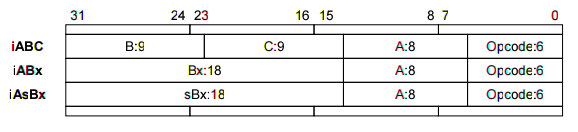
\includegraphics[scale=0.5]{luabytecode.png}
	\end{center}
 
  \caption[Lua VM bytecode layouts]{Lua VM bytecode layouts
    \protect\cite{RobertoIerusalimschy}}
  \label{fig:luabyte}
\end{figure}

With bytecode, the overhead of parsing the program is part of the
compilation step, which is separate from execution. This separation is
useful because the program can be parsed (and optimised) a single time
so no future execution of the program will have to incur the overhead
of parsing the source code.

Since the bytecode is simple, decoding which operation the VM must
perform and on which arguments is much faster than the kind of parsing
needed for a line of text. This means the VM can have fast startup and
fast execution. The bytecode is also more compact than the abstract
syntax tree representation.

Bytecode interpreters or virtual machines present a good solution for
an interpreter for general use by applications. More detail about the
the organisation of virtual machines follows.

\section{Organisation of a Virtual Machine} 
A virtual machine executes a file that is a list of instructions in
the bytecode format for that virtual machine. For the Lua VM these
instructions would be 32-bit integers in one of the formats seen in
Figure~\ref{fig:luabyte}. This file, called a binary file or simply a
program, is read by the virtual machine and its instructions are
followed. How exactly this occurs will be explained in further
chapters. The binary file must conform to the bytecode format for the
virtual machine, and may only make use of instructions found in the
instruction set of the virtual machine.

\subsection{Instruction Set}
Each VM has a set of subroutines called the instruction set. A
subroutine is a ``set of instructions designed to perform a frequently
used operation within a program'' \cite{ComputerWords}. An important
distinction here is critical to avoid confusion. The instruction set
of the virtual machine is a set of subroutines. These subroutines are
made up of instructions that the real (or host) machine executes.

Each of these subroutines in the VM's instruction set performs a
specific operation necessary for the execution of a program. A VM
usually has instructions for performing arithmetic operations
(\verb|add|, \verb|divide|, \verb|subtract| ...), bit manipulation
operations (\verb|xor|, \verb|and|, \verb|or| ...), control flow
operations (\verb|jump|, \verb|jump_if_zero|, ...) and for storing and
accessing values (\verb|load|, \verb|store|, ...). The design of a VM
instruction set, much like that of a CPU, is a creative process. The
particular set of instructions a virtual machine has is the decision
of the designer and choosing which instructions to include and omit
has trade-offs that need to be considered.

There are several classes of machine architecture and these are often
most easily distinguished by the form of their instruction
set. \textbf{Stack} machines often have instructions without operands,
\textbf{Accumulators} usually have instructions with a single operand,
and \textbf{Register} machines will usually have one to three operands
per instruction. These are also distinguished by the number of
registers each has.

In order for the VM to use its instruction set, it has to be able to
read the instruction from the binary file and then execute the correct
subroutine for that instruction. This process is called ``dispatch''
and each VM has some implementation of a dispatch mechanism.

\subsection{Dispatch Mechanism} 
At the core of the virtual machine is its dispatch mechanism. The
purpose of the dispatch mechanism is to move execution from the
current instruction to the next instruction in the program by
selecting the correct subroutine in the instruction set and executing
it. The VM reads the instruction that the instruction pointer points
to and then must determine what subroutine needs to be called to
execute the instruction. Selecting and moving execution to this
subroutine is called ``dispatch''. The implementation techniques for
instruction dispatch are important in this study. However, they are
technically complex and are therefore revisited in section
~\ref{sec:dispatch}. The dispatch mechanism also influences how the
opcodes in the instruction word are separated from the operand.

\section{Problem Description}
Modern process virtual machines make use of JIT compilers. Both JVM
and .Net make use of a JIT compiler \cite{MSDN,Oracle}. 

For applications that run many concurrent instances, like a web server
which starts up a new process for every client, a virtual machine that
makes use of a JIT compiler defeats the benefits of read-only memory
sharing. This is because jitted code is created at runtime and thus is
saved in the process's private memory. Jitted code is not shared
between instances of the VM running the same code.

Bytecode that has not been jitted can be shared between these
instances. In order to take advantage of read-only memory sharing a
JIT-less virtual machine is needed. However, as will be discussed in
chapter 2, JIT compilation can greatly reduce the time taken to
execute programs. Thus alternative ways to increase the performance of
the VM need to be found for the performance of a JIT-less VM to be
competitive.

\section{Project Objectives}
The objective of this project is to implement and benchmark an
experimental JIT-less virtual machine design for a dynamically typed
language. In order to benchmark the performance of the virtual machine
an additional two virtual machines must be developed. One of these is
a conventionally implemented virtual machine. The other is an
additional experimental VM needed to test the effectiveness of a
particular element of the proposed solution. This will be discussed
further in chapter 3.

A set of benchmarks must be hand-written to run on the new virtual
machines. The running times of the benchmarks on each of the three
virtual machines must be compared and analysed. The project aims to
determine what kind of performance benefits (if any) can be attained
by the two experimental implementations over the conventionally
designed virtual machine.

\section{Project Scope}

The VMs are experimental prototypes, hence several tools and features
conventionally paired with a VM are considered out of scope for this
project. There will be no \textbf{compiler} or \textbf{assembler}
implementation required and the VM will not be required to perform
\textbf{garbage collection}.

\begin{itemize}
\item A compiler implementation is unnecessary as the VM designs are
  experimental prototyped and are not meant for further use, thus
  benchmarks can be hand-written as they are the only programs needed
  to run on the virtual machine. Similarly, robust error handling and
  debugging tools are considered out of scope.
	
\item An assembler will be used to make writing benchmarks more
  bearable but is not considered in scope as it is simply a tool used
  to facilitate easier writing of benchmarks and not an important part
  of the implementation of the virtual machine.
	
\item Garbage collection is considered out of scope because the
  implementation of a garbage collector adds to the complexity of the
  project and may influence the results of running the benchmarks. A
  GC is also unnecessary to run the benchmarks.
\end{itemize}


%floating point and advanced threading techniques

\section{Risks}
A risk for any research project is to allow personal bias to cloud the
conclusions drawn from the results. This study aims to follow the
scientific method and disclose as much information as is necessary for
the study to be repeatable. The fact that the virtual machine is a
prototype that runs a known set of benchmarks means that there is a
risk of creating a virtual machine that is specialised for its own
benchmarks. The VM must have a design that provides good performance
generally and hence the set of benchmarks is diverse in order to
mitigate this risk.

A possible risk in the design of the study is that the hand-written
benchmarks may not be optimised as well as those produced by a
compiler. However, since all three VMs will run identical benchmarks
this risk is mitigated because any lack of optimisation in a benchmark
experienced by one VM will be experienced by all other VMs. Comparing
the experimental VMs with an existing conventional VM design would be
ineffectual as it may perform better purely because the code produced
by the compiler is better optimised.

\section{Overview of Treatise}
In chapter 2, the virtual machine as a concept will be introduced and
the different types of virtual machines will be covered. Existing
solutions to the problem of a VM for dynamically typed language will
be examined and some theory about modern processors will be
covered. This theory informs some of the design decisions of the
virtual machine.

In chapter 3, the design of the VM will be covered. This chapter will
cover how the VM works, what instructions it supports and discusses
why certain design decisions were made given the information in
chapter 2.

In chapter 4, the implementation details of the VM are covered, with
code samples provided as examples for various important elements of
the VM's design like dispatch, function calls and how instructions are
implemented.

In chapter 5, the experimental design and benchmarks will be
discussed. Which benchmarks were chosen and what they can tell us
about the virtual machine will be discussed in this chapter. It will
also detail the exact details of how the experiment was conducted so
that it may be repeatable with similar hardware.

In chapter 6, the results of the experiment will be discussed and
analysed and the performance benefits of the virtual machine will be
examined.

Lastly in chapter 7, conclusions will be drawn regarding in what
instances the experimental implementation of the virtual machine is
useful and what its strengths and weaknesses are.
\newpage{}

\chapter{Background, Literature Review and Existing System}
The term ``virtual machine'' is used to refer to a number of different
programs. Some virtual machines are designed to emulate real computers
and can have operating systems installed on them. Other virtual
machines exist only to run a single program to completion. In order to
disambiguate the term, a discussion of the hierarchy of virtual
machines follows, and the VM that is the focus of this study is
situated within it. This discussion follows in section
~\ref{sec:vms}. This is followed by a short discussion that outlines
the distinction between dynamically and statically typed languages.

In chapter 3, the design of the virtual machine is discussed. The
design decisions behind the virtual machine take into account how the
modern computer processor architecture works. Hence a discussion of
the modern processor architecture is necessary background information
that informs the decisions and trade-offs that are discussed in chapter
3. This discussion will follow in section
~\ref{sec:processor_architecture}.

Finally, in section ~\ref{sec:research} the current literature on
virtual machines is consulted for information about which VM designs
have proved effective in the past and what techniques are available
for various elements of the virtual machine's design.

\section{Virtual Machines}
\label{sec:vms}
A \textbf{virtual machine} or \textbf{VM} is a computer program that
``executes software in the same manner as the machine for which the
software was developed'' \cite[pg9]{JamesE.Smith2005}. This program is
designed to run on some real machine. We call the real machine that a
virtual machine is running on the \textbf{host} and the virtual
machine the \textbf{guest}. The guest machine provides an execution
environment for software that is designed to run either on the guest
itself or on an actual machine that the virtual machine is
emulating. This means that we can use a virtual machine to run
programs that are incompatible with the host. The virtual machine
allows this by providing a mapping of its state to the state of the
host machine on which it is running \cite[pg4]{JamesE.Smith2005}.

\subsection{The Types of Virtual Machines}
Virtual machines come in two varieties: \textbf{process} virtual
machines and \textbf{system} virtual machines. A process virtual
machine is ``capable of supporting an individual
process''\cite[pg9]{JamesE.Smith2005}. This means that the host runs
the guest for as long as a single process on the guest machine needs
it. Once the process has completed its execution the guest machine
terminates \cite[pg9]{JamesE.Smith2005}. An example of a process
virtual machine is the Java Virtual Machine or JVM. All Java programs
run on the JVM. An instance of the JVM is started when you execute a
Java program and terminated when its execution is complete.

A system virtual machine ``provides a complete system environment''
\cite[pg9]{JamesE.Smith2005}. This means that it can support an entire
operating system on the guest machine and the many processes that the
guest operating system executes. A system virtual machine will
terminate when the guest system is shut down.

This study focuses on process virtual machines and hence the finer
details of system virtual machines will not be discussed. In the class
of process virtual machines, however, there are further distinctions
to be made.

\subsection{The Types of Process Virtual Machines}

Process virtual machines can be divided into two categories:
\textbf{multiprogrammed systems} and \textbf{dynamic}
\textbf{translators}. The difference between these is whether or not
the guest machine uses the same instruction set architecture as the
host machine.

With multiprogramming the guest and host use the same instruction
set. Multiprogramming is supported by most operating systems and
allows a user to run many processes at once by ``making each process
think it has access to an entire machine instead of only part of a
machine'' \cite[pg13]{JamesE.Smith2005}. The OS creates an environment
per process that it terminates when that process ends execution.

With dynamic translators the instruction set of the host and guest
generally do not match. The virtual machine translates blocks of
instructions meant for the machine it is emulating and translates them
into instructions to be run on the host. Not all code is translated in
a dynamic translator. Only code that is used often enough will be
translated as there is an overhead involved with translating code. The
code that is not translated is interpreted. Interpreted instructions
are read, their meaning interpreted and then executed. This
interpretation step must happen each time a piece of code is executed
so code that is executed enough times will be dynamically translated
and cached so later execution is faster. Dynamically translating in
this manner is known as \textbf{just-in-time compilation} (JIT
compilation).

\subsection{Where the VM is Situated}
The VM is a process virtual machine. It has a new instruction set
architecture and hence is different from any host machine's ISA. The
VM is exclusively an interpreter and does not make use of a JIT
compiler. For this reason it is a ``JIT-less'' virtual machine. But
what is it that makes the virtual machine a ``Dynamic-ISA'' VM? A
dynamic ISA virtual machine is one used to interpret bytecode from a
dynamically typed language. One way of classifying programming
languages is by their type systems. There are two common type-system
approaches used by programming languages. These are dynamic typing,
used by dynamically typed programming languages and static typing
which is used by statically typed programming languages. These two
types of languages are now compared.

\section{Dynamic vs Statically Typed Programming Languages}
A dynamically typed language is one in which the type information is
associated with values \cite[pg4]{RobertoIerusalimschy}. An example of
a dynamically typed language is JavaScript. In JavaScript the
\verb|var| keyword is used for variables. This is because the type is
associated with the value stored in the variable so variables
themselves need not be told which type is associated with them. Any
variable can hold a value of any type. A statically typed language is
one in which the type information is associated with the variable. An
example of this is Java. In Java variables are declared using keywords
that define their type (\textbf{int}, \textbf{String} etc). Each
variable can only hold a value of that type. Each approach has its
strengths and weaknesses.

\subsection{Type Safety}
\label{sec:type_safe}
With static typing a program's type correctness can be checked at
compile time. Because the types of all variables are known when the
code is written, operations on those variables can be declared valid
or invalid when code is compiled. If an operation that acts on one
type of variable is given another, the program will not compile. This
knowledge is advantageous for the programmer and for the machine (or
VM as the case may be).

The programmer benefits from knowing whether or not his program is
correct at compile time. The implications of this are larger than just
being able to find errors while compiling some piece of code instead
of while running it. A type error in a dynamically typed language has
to actually be executed before it can be detected. If a type error
occurs in a rarely taken path of execution in a dynamically typed
program, it may not be detected at all. This means that a programmer
writing in a dynamically typed language must ensure that the values in
the variables they use are of types that make sense for the operations
they wish to perform. A programmer writing in a statically typed
language will have his types checked for him.

The machine or VM benefits from not having to check the types of
instruction arguments. This is a major overhead in dynamically typed
languages. In a dynamically typed language, the types of the arguments
must be checked for each instruction the VM or machine must perform as
the arguments of the instruction could be of any type the VM
supports. This means that an addition instruction that works on
integers, for instance, must check that the values it is trying to add
are in fact integers before it can add them.

Figure \ref{fig:dvs} shows how Java, a statically typed language
and Lua, a dynamically typed language, handle code which tries to
perform addition of two types that cannot be added in either
language. The Lua code compiles but encounters an error at
runtime. The Java code does not compile.

\begin{figure}
	\begin{subfigure}{.48\textwidth}
		\begin{lstlisting}[numbers=none,frame=none]
class main {
    public static void main(String[] args) {
        int foo = 12;
        String bar = ``bar'';
        int foobar = foo + bar;
    }
}
		\end{lstlisting}
		\caption{Java: does not compile}
	\end{subfigure}
	\begin{subfigure}{.48\textwidth}
		\begin{lstlisting}[numbers=none,frame=none]
foo = 12
bar = ``bar''
foobar = foo + bar
		\end{lstlisting}
		\caption{Lua: compiles but encounters error}
	\end{subfigure}
	\caption{Dynamically vs Statically Typed Languages}
	\label{fig:dvs}
\end{figure}

\subsection{Advantages of Dynamically Typed Languages} 
Dynamically typed languages have their own advantages. Programs
written in dynamically typed languages tend to be shorter than
equivalent programs written in statically typed languages and
dynamically typed languages are considered to be easier to prototype
ideas in. Also, a subset of logically correct programs will not be
accepted by a statically typed language's type checker. Dynamic typed
languages allow the freedom to write these kinds of programs.

Dynamically typed languages are also powerful for handling arbitrary
data. This is exemplified by the JSON format, based on a subset of the
dynamically typed language, JavaScript. JSON is used as a language
independent, data-interchange language \cite{JSON}. In JavaScript,
objects that can contain arbitrarily arranged data can be created
during runtime, while in most statically typed languages, classes that
commit the programmer to specific formats for data must be
defined. The C\# programming language includes a ``dynamic'' type
\cite{dynamic} that allows programmers to work around this limitation
of statically typed languages.

Of course statically and dynamically typed languages can be realised
in many different ways, but currently both dynamic and statically
typed languages are widely used and so research for both statically
and dynamically typed languages is important.

Since virtual machines are a platform on top of which other programs
must run, the performance of the VM itself affects the performance of
every program that runs on it. An understanding of the hardware that
the virtual machine runs on is necessary to optimise the performance
of the virtual machine. A summary of the aspects of the processor
architecture important for virtual machine performance follows.

\section{Modern Processor Architecture}
\label{sec:processor_architecture}

In order to create an efficient VM, we need first understand how
modern processors work and what some of the bottlenecks for our VM's
execution might be. For example, \textbf{threading techniques} (not to
be confused with threads in application programming) are commonly used
in VM design. These take advantage of a feature of modern processors
called the \textbf{Branch Target Buffer} or BTB. The BTB exists to aid
a process called \textbf{branch prediction}. Branch prediction itself
can only be explained once we know about how modern processors make
use of \textbf{pipelining} to increase their throughput. As you can
see, an understanding of modern computer architectures is needed
before we can begin a discussion of VM design.

\subsection{Pipelining}

Pipelining is a process in which a processor's instruction processing
cycle is shared by many consecutive instructions at once. The
instruction processing procedure is split up into smaller stages that
can execute simultaneously. An example of this is the classic RISC
pipeline which divides instruction processing into the following
steps: Instruction Fetch (IF), Decode (ID), Execute (EX), Memory Access
(MEM) and Writeback (WB). Each instruction passes a stage and leaves
that part of the processor free to perform that stage on the next
instruction. Thus many instructions (as many as there are stages) can
be processed at once, instead of each instruction having to be
completely processed before the processor is free to move onto the
next instruction. This process is analogous to an assembly line, where
many cars can be assembled at the same time, each in a different stage
of assembly.

\begin{figure}[tph]
  \centering
  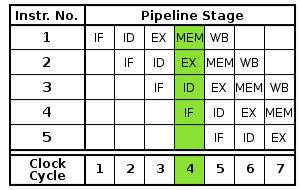
\includegraphics[scale=0.5]{pipeline}
  \caption[Simplified CPU pipeline]{Simplified CPU pipeline \cite{pipeline}}
  \label{fig:pipeline}
\end{figure}

In figure~\ref{fig:pipeline} the first instruction as
currently performing memory access while the second EXecutes and the
third is being Decoded. Up to 5 instructions can be processed
simultaneously in this system.

When pipelining an interesting situation occurs in the case of some
control flow instructions. Control flow instructions are those that
cause execution to move to some other point in the program. For
control flow instructions where the jump is conditional (based on some
criteria being true) the point at which we know which instruction
comes next (called \textbf{branch resolution}) is usually later in the
pipeline. Thus the processor cannot queue up the next instruction as
it does not know which instruction will execute next. Branch
prediction is used in modern processors to try to keep the pipeline as
full as possible and not waste time waiting for this information to be
known.

\subsection{Branch Prediction}

Instead of filling up the pipeline with no operation instructions
until we know where to branch, with branch prediction we guess which
branch will be taken and place the instructions from the predicted
branch into the pipeline. When we know where the branch operation
should have taken execution we either throw out our newly pipelined
instructions (this is called \textbf{pipeline flushing}) if the
prediction was incorrect or continue execution if it was correct.

The more stages the pipeline has before branch resolution, the more of
a performance benefit correct predictions become for programs with
many conditional control flow instructions. A Virtual Machine is such
a program. This is because a VM must branch to the correct code for
each instruction it executes. Writing code that allows for increased
branch prediction accuracy is thus important for VM efficiency.

Predicting a branch means we must predict if that branch is taken or
not and what the target of that branch is if it is taken. Modern
processors have a Branch Target Buffer where the target adresses of
previously taken branches are cached. So upon arrival at a branch that
has been previously taken, we guess if it will be taken and begin
speculatively executing from the address stored in the BTB.

\subsection{Cache}
\label{sec:cache}
Modern processors make use of different levels of cache to allow for
faster memory access. Ideally we would like to have an infinite amount
of memory with no time cost for accessing it. The reality is that the
larger memory is, the slower it becomes to access it. In order to get
closer to the ideal modern processors make use of cache. It takes
around 100 cycles for Intel's i7-4720HQ (Haswell) architecture to
access memory. Cache allows us get get closer to the ideal case by
keeping commonly accessed memory closer to the CPU in levels of
increasingly smaller, faster and more expensive (to manufacture)
memory. 

The Haswell architecture has 32KB of L1 data cache and 32KB of L1
instruction cache. These are located on the CPU itself. L1 data cache
can be accessed in around 4 cycles \cite{7-cpu}. It also has 256KB of
L2 cache and 8 MB of L3 cache. L2 cache can be accessed in 12 cycles
and L3 in about 36 cycles \cite{7-cpu}. Caching works on the principal
of locality of reference. There are two types of locality of
reference: spacial locality and temoporal locality.

Temporal locality takes advantage of the likelihood that similar data
will be needed in the near future. If some data has been accessed
recently it is cached because it is quite likely it will be needed
again soon.

Spacial locality takes advantage of the likelihood that similar data
will be needed in the near vicinity of an accessed value. Data near an
accessed value is cached because it is likely that it will be
needed. This would be good for something like sequential array lookups
because more of the array will be cached for faster access later. With
knowledge of how cache functions a VM that makes effective use of the
processor's cache can be implemented.

\section{Conventional Implementation of High Level VMs}

Several common patterns are found in the design of Virtual
Machines. Different techniques for threading the flow of execution
through the VM have been well-examined and the trade-offs between
register and stack-based VMs have been discussed and studied.

\subsection{Decoding Instructions}
\label{sec:decode}
Conventional virtual machine design requires that instructions are
decoded before they can be executed. The tasks of decoding the
instruction are to extract the opcode and operands from the current
instruction word. This decode step must happen before each
instruction can be executed. 

As an example, the Lua bytecode is revisited in figure
\ref{fig:luabyte-repeat}. This image is the format for instructions
for the Lua VM. Instructions in the Lua bytecode are 32-bit
integers. Different sections of this 32-bit integer are used to encode
the opcode and operands.

\begin{figure}[!htb]
	\begin{center}
	    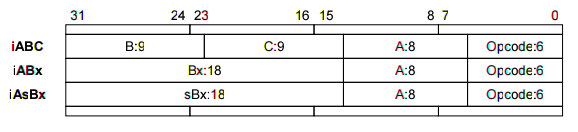
\includegraphics[scale=0.5]{luabytecode.png}
	\end{center}
 
  \caption[Lua VM bytecode layouts]{Lua VM bytecode layouts
    \protect\cite{RobertoIerusalimschy}}
  \label{fig:luabyte-repeat}
\end{figure}

The opcode, stored in the lowest six bits is extracted from the
instruction word first \cite{Lua.Source} and its value is used to jump
to the correct subroutine for that opcode. Then, each instruction that
takes arguments extracts opcodes from the 32-bit instruction word
using one of the three formats shown in the figure.

\subsection{Dispatch and Threading}
\label{sec:dispatch}
Dispatch is the process of fetching, decoding and starting the next
instruction to be run by a virtual machine.

The simplest way to implement a virtual machine is to make use of a
switch statement in a loop. This is called switch dispatch. See
figure~\ref{fig:switch} for a C implementation.

\begin{figure}
  \begin{lstlisting}
typedef enum { add /* ... */ } Inst; 

void engine() 
{ 
    static Inst program[] = { add /* ... */ }; 
    Inst *ip = program; 
    int *sp; 

    for (;;) 
        switch (*ip++) 
        { 
        case add: 
            sp[1]=sp[0]+sp[1]; 
            sp++; 
        break; 
        /* ... */ 
    }
} 
  \end{lstlisting}
  \caption[Switch Dispatch]{Switch Dispatch\cite{Ertl}}
  \label{fig:switch}
\end{figure}

This approach is problematic because the switch statement means that
there is only ever a single entry in the Branch Target Buffer used for
indirect branches. This means that the number of mispredictions will
be large as the target of the branch will change for each new
instruction that the virtual machines branches to. This problem may
even be magnified by the fact that this specific VM implementation has
far more instructions than usual as it requires several specialised
versions of every instruction.

\begin{comment}The name threading comes from the idea of the execution
  threading its way from one instruction to the next {[}??{]}
\end{comment}

A faster alternative to switch dispatch is direct
threading\cite{Ertl}. In direct threading the program is stored as a
list of addresses of instructions and the code for each instruction
includes a dispatch portion which jumps to the address of the next
instruction to be executed.

\begin{figure}
  \begin{lstlisting}
typedef void *Inst; 

void engine() 
{ 
    static Inst program[] = { &&add /* ... */ }; 
    Inst *ip = program; 
    int *sp; 
    goto *ip++; /* dispatch first VM inst. */ 
add: 
    sp[1]=sp[0]+sp[1]; 
    sp++; 
    goto *ip++; /* dispatch next VM inst. */ 
}
  \end{lstlisting}
  \caption[Direct Threaded Dispatch]{Direct Threaded Dispatch\cite{Ertl}}
  \label{fig:direct}
\end{figure}

Another method is token threading. In token threading a lookup table
of the addresses of code for each instruction is kept and each
instruction dispatches to the next by reading the opcode of the next
instruction from the program, looking up the address of the code for
that instruction in the table and then jumping to that instruction.

\begin{figure}
  \begin{lstlisting}
typedef void *Inst;
void engine() 
{ 
    static Inst lookup[] = { &&add, &&sub /*...*/ }
    static int program[] = { 0, /* ... */ }; 
    int *ip = program; 
    int *sp; 	
    goto *ip++; /* dispatch first VM inst. */ 
add: 
    sp[1]=sp[0]+sp[1]; 
    sp++; 
    goto lookup[*ip++]; /* dispatch next VM inst. */ 
}
  \end{lstlisting}
  \caption[Token Threaded Dispatch]{Token Threaded Dispatch\cite{Ertl}}
  \label{fig:indirect}
\end{figure}

Direct and indirect threading make much better use of the branch
target buffer. Instead of a single entry in the BTB, with direct
threading we have an entry per instruction, so instructions that
commonly follow each other have a better chance of being predicted.


\subsection{Registers vs Stacks}
In a stack virtual machine, instructions act on members of the
stack. Arguments and return values for instructions are often implicit
and thus instructions can be smaller. For instance a stack
implementation of a = b + c would first push b and c onto the stack,
then call the add instruction which has no arguments. Add pops b and c
off the stack and pushes b+c back onto the stack. This value is then
popped off the stack and stored.

For a register machine, a similar piece of code would have values for
b and c in registers and an add instruction is called with a, b and c
as arguments. This instruction would compute b+c and store it in a
register.

Widely used process virtual machines make use of a stack
architecture. Both the Java Virtual Machine (JVM) and Microsoft's
Common Language Runtime (CLR) make use of stack virtual machines
\cite{CLI}\cite{JVM}.

\subsection{Just in Time Compilation}

Both the Hotspot Java Virtual Machine and .Net Common Language Runtime
make use of Just in Time compilation \cite{JVMJIT} \cite{CLRJIT}. JIT
compilation allows for code that is executed often enough to be
compiled into native machine code at runtime. This means that the
areas of code most frequently executed in the program run much faster
than they would otherwise and the overhead of compiling and optimising
every single piece of code, even that which is not used often, is
removed. Removing this overhead is important because slow compilation
at runtime can have a visible effect for users.

\section{Literature and Existing Systems}
\label{sec:research}

\subsection{Threaded Code}

James R. Bell introduced the concept of threaded code in 1973. The
Fortran IV compiler was written to generate threaded code.\cite{Bell}
Yuhne Shi\cite{Shi2007} found that a well-implemented register VM is a
more efficient option when speed of execution is more important than
the size of the code to be executed.

Ertl and Gregg found that in their benchmarks 3.2\%\textendash 13\% of
all executed instructions were indirect branches and that switch
dispatch on an architecture with a BTB resulted in 81\%-98\% branch
prediction misses \cite{EfficientInterpreters}. They also found that
direct threading resulted in 50\%-63\% branch prediction misses.

\subsection{Abstraction Level}
\label{sec:abstraction-level}
A 2009 study\cite{Brunthaler20093} by Stefan Brunthaler classed
virtual machines as high or low abstraction level virtual machines,
where low abstraction virtual machines are ``only a thin layer above a
real machine'' and high abstraction level virtual machines where the
``operation implementation requires significantly more native
instructions than for low abstraction level''.

The study aimed to question the established thought that instruction
dispatch was the main overhead for a virtual machine. He found that
this assumption does not hold for high abstraction level VMs, but is
valid for VMs with a low abstraction level.

\subsection{Specialised Instructions}

Michael Schr{\"o}der implemented a modified version of the Lua Virtual
machine that made use of the approach of specialising instructions
based on the types of their arguments when they are first
dispatched. In order to allow this to be safe, instructions that may
change the type of the arguments for that instruction have type checks
that will despecialise the instruction if need be. This approach
achieved a 20\% speed increase on Intel machines\cite{Schroder2012}.

\subsection{Existing Systems}

The Lua VM is an interpreter for the dynamically typed language Lua's
bytecode. Lua is used as a scripting language in game engines
\cite{LuaUsed}. It has many implementation similarities to the VM
described in this treatise and thus is of particular interest but it
differs in its strict adherance to the ANSI C standard
\cite{RobertoIerusalimschy}. Strict adherance to the standard is
something prioritised by the Lua team for portability reasons
\cite{RobertoIerusalimschy}.
\begin{description}
\item[Dynamically typed] Lua's types are associated with its values
  and not its variables.
\item[Register-based] The Lua VM is register-based instead of the
  stack approach taken by the JVM and .NET runtime.
\item[Switch Dispatch] The Lua VM makes use of the a switch dispatch
  mechanism \cite{Lua.Source}. This is a result of its strict
  adherance to the ANSI C standard which does not allow for labels as
  values which are needed for alternative threading techniques.
\item[No JIT] The lua VM does not make use of a Just in Time compiler
  (though an independent project called luajit has provided one).
\end{description}

\subsection{HotSpot JVM and .NET runtime}
Oracle's Java Virtual Machine implementation, called HotSpot is a
high performance Virtual Machine for running java
bytecode. Microsoft's .NET runtime is a similar VM that runs the
common intermeidate language that several Microsoft-developed
languages compile to. They are implemented similarly to each other and
quite differently from the VM described in this treatise:
\begin{description}
\item[Statically Typed] Both VMs make use of static types. Types are
  associated with variables instead of values.
\item[Stack-based] Both are stack-based architectures instead of
  register-based
\item[JIT] Both VMs make use of Just in Time compilation.
\end{description}

\subsection{Dalvik VM}
The Dalvik VM executes applications written for Google's Android
operating system for phones and tablets. The common is is that JVM
bytecode is translated to Dalvik bytecode to run on the Dalvik
VM. Dalvik has been replaced by ART in Android 5.0. Unlike the JVM,
the Dalvik VM is a register machine.
\begin{description}
\item[[Statically Typed]] Dalvik VM bytecode is statically typed
\item[Register-based] The Dalvik VM makes use of a register-based
  design
\item[JIT] Dalvik VM code is jitted
\end{description}

\chapter{Solution Design}
This study introduces two experimental virtual machines. \textbf{The
  Operand Dispatch VM} and the \textbf{Operand-Type Dispatch VM}. The
two central ideas behind these experimental virtual machines are
type-mapping and operand case expansion. The Operand Dispatch VM makes
use of operand case expansion exclusively. The Operand-Type Dispatch
VM however, makes use of both operand case expansion and type
mapping. 

It may be tempting to propose a third virtual machine that makes use
of type-mapping exclusively and does not use operand case expansion,
but type-mapping cannot be decoupled from operand case
expansion. Operand case expansion is necessary to implement a
type-mapped VM. These two techniques, operand case expansion and type
mapping will now be discussed.


\section{Type-Mapping and Operand Case Expansion}
\label{sec:type-mapping-op-case-exp}
A type-mapped VM is one which keeps track of the state of the types of
its registers. This is called the type-state of the virtual
machine. This is beneficial because, as was discussion in section
\ref{sec:type_safe}, every instruction in a dynamically typed VM
must first verify the types of its inputs before it can act on
them. These type checks can be eliminated with type-mapping. Another
benefit of type-mapping is that instructions can be specialised based
on the current type-state of the virtual machine.  

Operand case expansion unrolls the instruction set of a virtual
machine into a set of operand-specific versions of every
instruction. An example can be seen in figure
\ref{fig:op-case-expansion}. In this instance an \verb|add|
instruction for a virtual machine with n registers is expanded into
$n^2$ different instructions for each operand case. Operand case
expansion is beneficial because it removes the decode step present in
a conventional virtual machine design (see section
\ref{sec:decode}). This is because the entire instruction word can be
used to select the specific version of the instruction needed. The
implementation details of operand case expansion is examined in chapter 4. 

\begin{figure}
	\centering
	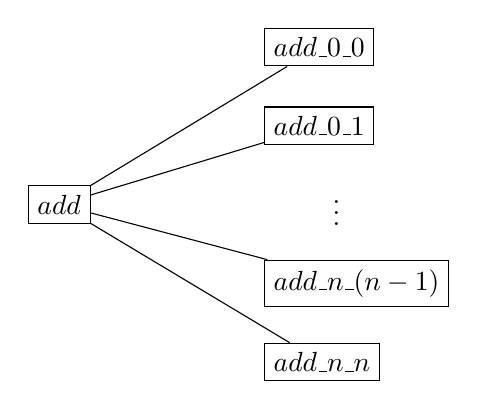
\begin{tikzpicture}
	\tikzstyle{every node}=[draw,shape=rectangle,anchor=west];
	\node (v0) at (0,-2) {$add$};
	\node (v1) at (3,0) {$add\_0\_0$};
	\node (v2) at (3,-1) {$add\_0\_1$};
	\node[draw=white] (v3) at (3.75,-2) {$\vdots$};
	\node (v4) at (3,-3) {$add\_n\_(n-1)$};
	\node (v5) at (3,-4) {$add\_n\_n$};
	\draw (v0) -- (v1)
	(v0) -- (v2)
%	(v0) -- (v3)
	(v0) -- (v4)
	(v0) -- (v5);
	\end{tikzpicture}
	\caption{Operand Case Expansion}
	\label{fig:op-case-expansion}
	
\end{figure}

Type-mapping is closely coupled with the idea of argument case
expansion. For type-mapping to work, the VM must dispatch on its
current type-state. But if the VM does not also dispatch on the
operands for the next instruction it cannot know which version of the
instruction is appropriate. Knowing which types are in which registers
without knowing which registers are arguments for an instruction means
that there is not enough information to specialise the instruction.

\section{Proposed Solution}
The proposed solution is the Operand-Type Dispatch VM which makes use
of type-mapping and argument case expansion. In order to determine the
effectiveness of the solution, a further two virtual machines are
needed. A conventionally implemented virtual machine is needed as a
control to determine the performance benefits of the Operand-Type
Dispatch VM and a further VM is needed to determine the benefits of
the type-mapping of the Operand-Type Dispatch VM over just using
argument case expansion.

These three virtual machines lie along a scale for how specific their 
instructions are. The most specific is the Operand-Type Dispatch VM. 
The Operand Dispatch VM is less specific and the Conventional 
Dispatch VM has the least specific instructions.

The details of the designs of these three virtual machines is
discussed from section \ref{sec:conv-vm} after design decisions common
to all VMs have been introduced. The three virtual machines are
designed to be as similar as possible except for the aspects that the
experiment examines. Those elements common to all VMs are expanded
upon first and those specific to each shall be examined separately.

Any referral to the \textbf{VM} or the \textbf{virtual machine} used
from this point without explicitly mentioning which VM is being
referred to will apply to \emph{all} three virtual machines.

\section{Virtual Machine Design Details}

The VM is a register virtual machine. The choice of being
register-based is necessary for the operand case expansion to be
performed. Of course, since type-mapping requires operand case
expansion, that also necessitates that the virtual machine use
registers. Yuhne Shi\cite{Shi2007} showed that register machines can
give a performance increase over equivalent stack-based VMs. This
makes them an ideal choice for a performance-focused virtual machine
design.

\subsection{Registers and Implicit Assignment}
The VM has six general purpose registers and three special purpose
registers. A low number of registers adds complexity to a potential
compiler for this virtual machine because the compiler must perform
register allocation more frequently, but keeping the number of
registers low is important for the Operand-Type Dispatch and Operand
Dispatch VMs. This is because a large number of registers would
greatly increase the number of operand cases needed to implement
instructions that take register arguments. With just six registers, an
instruction that takes three arguments potentially has $6^3 = 216$
operand cases. With 10 registers, that would be $10^3 = 1000$.

Because every argument in an instruction increases the number of
operand cases exponentially, where possible, instructions in the VM
include an implicit assignment. That is, instead of having an
instruction, \verb|add g1, g2, g3|, which adds \verb|g2| to \verb|g3|
and stores the result in \verb|g1|, the VM implements the \verb|add|
instruction as follows: \verb|add g1, g2|. This instruction adds
\verb|g1| to \verb|r2| and stores the result in \verb|g1|. In this way
the number of operand cases can be kept reasonably low. The
Operand-Type Dispatch VM faces a similar issue that affects the
decision for which types the VM should use.

\subsection{Types}

The VM has two primitive types: integers and pointers. Keeping the
number of types low is extremely important for the Operand-Type
Dispatch VM because it affects the total number of states the VM can
take on. The Operand-Type Dispatch VM can be thought of as creating a
specialised version of the VM for every type state. With two primitive
types and six registers this means there are a total of $2^6 = 64$
total states the VM can take on. Increasing the number of primitive
types by one makes that $3^6 = 729$ possible states.

The decision to have only two types was made because of the increased
complexity that would be associated with an additional type. Floating
point numbers were considered as a third type for the virtual machine,
but this would add considerable complexity to the implementation of
the virtual machine. This is because arithmetic instructions in the
virtual machine would now have to act on two different types and on
the different combinations of those two types.

\subsection{Values} 

A register virtual machine for a dynamically typed language must be
able to hold any type of value in any of its registers. This is the
reason the type checking operations explained in section
\ref{sec:type_safe} must take place. The VM registers are used to
store \textbf{values}. Values are a convenient data structure that can
hold either a pointer or an integer, as these are the types supported
by the VM. The implementation details of values are covered in section
\ref{values-implementation}. Most instructions in the VM take
arguments which are general purpose registers which hold values, but
two other modes of addressing exist in the VM.

\subsection{Addressing}
Instructions take operands of three types: 
\begin{description}
\item[register number] These operands are numbers from 0 to 5 that
  address the six registers. For the conventional VM these operands
  are an explicit part of the instruction word. For the Operand-Type
  and Operand Dispatch VMs these operands are implicitly part of the
  instruction word. Implementation details of register number
  addressing will be discussed in chapter 4. %TODO section??
\item[instruction word] This type of operand considers an instruction
  word relative to IP (usually just the next instruction word) as an
  unsigned 16-bit constant. The value of these constants will be
  referred to in the following form: $name_{16}$
\item[IP-relative addressing] This type of operand considers an
  instruction word as the \verb|IP|-relative address of a 64-bit
  unsigned integer constant. The 64-bit integers accessed by
  IP-relative addressing are aligned to 8-byte addresses. The value of
  the 64-bit constant will be referred to in the following form:
  $name_{64}$
\end{description}

Instruction word addressing is used when large integer values are not
needed. This is the case, for instance, when performing a left shift
by a known constant. Shifting a 64-bit integer left by anything more
than 63 bits will always result in a zero value and so a larger
integer value is not needed. IP-relative addressing is used when a
larger value may be needed. An examination of the instruction set of
the VM follows:

\section{Instructions}

All three virtual machines provide a set of 46 instructions. These
shall be referred to as ``logical instructions'' as they enumerate the
entire set of functions the VMs can perform. All VMs provide the same
functionality. These 46 instructions make up the set of possible
instructions that can exist in an unassembled program for any of the
three virtual machines. 

For each VM, however, there are different implementations of these
logical instructions. For the conventional VM, there is a single
``internal instruction'' for each of the 46 logical instructions the
VM provides. It has a one-to-one correspondence between logical an
internal instructions. 

For the Operand-Type and Operand Dispatch VMs there are, in some
cases, multiple internal instructions for each logical
instruction. For these cases, there is a many-to-one correspondence
between the internal instructions and the logical instructions they
implement.

\subsection{Instruction Set Design Factors}
\label{sec:inst-set-design-factors}
In some cases, specific argument combinations for a logical
instruction have been removed as they produce trivial results. For
instance the subtract operation cannot be used with the same register
for both arguments. Since the result of this operation is always zero
and there already is an instruction to set a register to zero, there
is no need to include this case.

The VM instruction set design was made with memory hierarchy of modern
computers in mind. The instruction set is designed to be as robust and
general as possible. The aim is for the instruction subroutines needed
by the VM to be in L1 instruction cache. The VM has an instruction set
of 46 instructions. Because of the operand case expansion the Operand
Dispatch VM has 1295 internal instructions. The Operand-Type Dispatch
VM has 2021 internal instructions and a special instruction to signal
an error. The difference ($2022 - 1295 = 728$) is the set of type
specialised internal instructions.

A rough estimate of the size of a low abstraction level
\cite{Brunthaler20093} internal instruction for the Operand VM is 120
bytes. This means the Operand VM would requires around 151KB of cache
to house the entire instruction set. The Haswell processor, as
mentioned in section \ref{sec:cache}, has 32KB of L1 instruction
cache. Only a small fraction of the instruction set will be in use at
any time. This must be the case, because 720 of the 1295 instructions
in the Operand-Dispatch VM are used to implement four logical
instructions: \verb|geto|, \verb|seto|, \verb|getb| and
\verb|setb|. 

The Operand-Type VM's low abstraction level internal instructions are
approximately 60 bytes. This works out to only 118KB of instruction
cache needed for the entire instruction set.

The size of the instruction set in cache is not the only issue to
consider for the Operand and Operand-Type Dispatch VMs
however. Associated with each of these virtual machines is a lookup
table used for their dispatch mechanism. The dispatch mechanism of
each VM is discussed in section \ref{sec:labels-as-addresses}. This
lookup table is referred to as the \textbf{dynamic opcode table}.

The dynamic opcode table is a set of 8-byte pointers. In the Operand
Dispatch VM, the dynamic opcode table is $(1296*8)/1024 = 10$KB, a
fraction of the L1 data cache for a Haswell processor. For the
Operand-Type dispatch however, the lookup table is
$(131072*8)/1024 = 1$MB which is around 30 times larger than L1 data
cache. This is less of a problem than it seems. Firstly, 36.7\% of
this table is never used. A further 42.4\% of the table entries are
only used if there is a type error, in which case the program's
execution will not complete anyway. Furthermore only a small fraction
of the remaining 20\% (which could fit in L2 cache on a Haswell
machine) of the table is actually used by a single program.

A sample of the instructions provided by the VM follows. The full set
of instructions may be found in appendix B.

\subsection{Arithmetic Instructions}

Arithmetic instructions provide basic arithmetic operations for
registers that contain integers. If a register that does not contain
an integer is selected, an error is signalled and the VM halts. All
arithmetic instructions increment the address of the instruction
pointer. Those that make use of a constant that is looked up in the
next instruction word increment the instruction pointer's address
again so that the \verb|IP| points to the next instruction and not the
data contained in the next word.

\begin{description}
	\item[sub] find the difference of two integer-valued registers
	
	$sub(i, j\neq i) := r _{i} \longleftarrow  r _{i} - r _{j} $ \\	
	
	\item[addc] add an integer-valued register and a 64-bit integer
	constant
	
	$addc(i, const _{64}) := r _{i} \longleftarrow  r _{i} + const 
	_{64} $ \\
\end{description}

The \verb|sub| instruction exhibits the case of a trivial instruction
call that is illegal in the bytecode. Subtracting a register's value
from itself will always produce zero. This is an unnecessary
instruction since the VM already has an instruction to place zero into
a register.

Both instructions also show off how the result of the operation is
stored in the first register-number addressed register.

\subsection{Bit Manipulation Instructions}

These instructions are for performing bitwise logical operations on
integer operands and constants. The \verb|IP| is incremented in the
same manner as for the arithmetic instructions.

\begin{description}
	\item[xor] bitwise xor two integer-valued registers
	
	$xor(i, j \neq i) := r _{i} \longleftarrow  r _{i} \textbf{ \^{} 
	} r _{j} $ \\
	
	\item[shrc] logical right shift an integer-valued register by a 
	16-bit
	integer constant
	
	$shrc(i, const _{16}) :=  r _{i} \longleftarrow  r _{i} >> const 
	_{16} $ \\	
\end{description}

Here we see another trivial case. The \verb|xor| instruction does not
allow performing bitwise xor on two numbers that are the same as this
value is always zero.

The \verb|shrc| instruction makes use of a 16-bit instruction word
after the instruction for the constant argument as a 64-bit argument
is unnecessary.

\subsection{Data Movement Instructions}
These instructions allow for values to be moved between registers.

\begin{description}
	\item[mov] move a register over another register
	
	$mov(i, j \neq i) := g_{i} \longleftarrow g_{j} $ \\
	\item[movc] move a 64-bit integer constant over a register
	
	$movc(i, const_{64}):= g_{i} \longleftarrow const_{64} $ \\
\end{description}

Note the use of the \verb|g| for the \verb|mov| and \verb|movc|
instructions. This is because moving a register over another register
is a type-independent operation.

\subsection{Memory Access}
These instructions allow for getting and setting of locals (getl,
setl), objects (geto, seto) and buffers (getb, setb).

\begin{description}
	\item[getl] get a local value indexed by a 16-bit integer 
	constant and store it in a register
	
	$getl(i, const_{16}):= g_{i} \longleftarrow mem[fp + const_{16}]$ 
	\\
	\item[seto] set a value, indexed by an integer-valued register, 
	in an
	object to that of a register
	
	$seto(i, j \neq i, k):= p_{i}[header + r_{j}*scale] 
	\longleftarrow g_{k}$ \\
	
	
\end{description}


\subsection{Control Flow Instructions}

These instructions allow for jumps in execution in the program. All
jumps are relative to the current \verb|IP| value.

\begin{description}
	\item[jmp] adds a 16-bit integer constant offset to \verb|IP|
	
	$jmp(const_{16}) := ip \longleftarrow ip + const_{16}$ \\
	\item[jmpf] adds a 64-bit integer constant offset to \verb|IP|
	
	$jmpf(const_{64}) := ip \longleftarrow ip + const_{64}$ \\	
	
	\item[jcmp] adds one of three 16-bit integer constant offsets to
	\verb|IP| depending on which case holds for two different
	integer-valued registers
	
	$jcmp(i, j\neq i,less_{16},equal_{16},greater_{16}) :=$ \\
	$ ip \longleftarrow  \\
	case :r_{i} < r_{j}: ip + less_{16}   \\
	case :r_{i} = r_{j}: ip + equal_{16} \\
	case :r_{i} > r_{j}: ip + greater_{16}$ \\
\end{description}


\subsection{Function Call and Return}

The function call mechanism was designed to be simple. Instruction
arguments must be stored contiguously in local variables in the
caller, and are copied as a unit into the local varaibles in the
caller. This mechanism may cause issues when multiple calls are needed
that require the same variables in different orders, but since the VM
is only to be used for a small set of benchmarks, these issues can be
avoided. This mechanism was chosen because it is an extremely simple
way to pass arguments. The function call mechanism saves registers
$g_1$ through $g_4$ before the function call. More detail on the
implementation of the function call and return mechanisms will be
given in section XXX.


\subsection{Pragmatic Higher-Level Instructions}

\begin{description}
		\item[newb]{} allocates a new object of size given by an
		integer-valued register and assigns it to some register
		
		$ newb(i, j \neq i) := $ \\
		$  object *base \longleftarrow (buffer*)malloc(sizeof(object) + 
		sizeof(int8\_t)* r_j) \\
		base.size \longleftarrow r_i\\
		g_i \longleftarrow base \\ $
		
		\item[out] writes out a stream of data from a buffer to stdout
		
		\item[print] writes a line of data to stdout
\end{description}

The aspects of the three virtual machines that set them apart from
each other are now discussed.

\section{Conventional VM Design}
\label{sec:conv-vm}

The Conventional VM makes use of a conventional decode step for each
instruction executed by the VM. The opcode and register-number
addressed operands are decoded from each instruction word using a
process of shift and mask operations. The layout of the conventional
VM's instruction words can be see in figure~\ref{fig:convinstruction}.

The two most commonly accessed parts of the instruction word, the
opcode and first argument are on each end of the instruction
word. This means that the opcode, on the left, need only be shifted
right to acquire its value. The first argument, on the right, need
only have the other bits masked. All other arguments require both a
mask and a shift operation.

\begin{figure}[!htb]
  \centering
	\begin{bytefield}[bitwidth=1.5em,endianness=big]{16}
	\bitheader{15,9,8,6,5,3,2,0} \\
    \bitbox{7}{opcode} & \bitbox{3}{arg3} & \bitbox{3}{arg2} & \bitbox{3}{arg1}\\
  \end{bytefield}
  \caption{Conventional VM instruction layout}
  \label{fig:convinstruction}
\end{figure}

All virtual machines make use of token-threaded dispatch as discussed
in \ref{sec:dispatch}, however the details of this dispatch are
slightly different for the three virtual machines and so will be
discussed separately. The Conventional VM dispatches exlusively on the
opcode section of the next instruction word. That is, the next
instruction word's opcode is decoded and is used to gain the address
of the subroutine needed for the next instruction. The implementation
details of the Conventional VMs dispatch mechanism are discussed in
section \ref{sec:conv-vm-dispatch}.


\section{Operand Dispatch VM Design}
The Operand Dispatch VM does not make use of the conventional decode
step present in the Conventional VM. This is a product of operand case
expansion. Figure \ref{fig:op-dispatch-instruction} shows the layout
of an instruction word for the operand dispatch VM. 

\begin{figure}[!htb]
  \centering
	\begin{bytefield}[bitwidth=1.5em,endianness=big]{16}
	\bitheader{15,0} \\
    \bitbox{16}{opcode with operands} \\
  \end{bytefield}
  \caption{Operand Dispatch VM instruction layout}
  \label{fig:op-dispatch-instruction}
\end{figure}

The Operand Disptach VM's entire instruction word is used for
dispatch. The combination of the opcode and the specific operand case
for that opcode is an index into the dynamic opcode lookup table for
token-threaded dispatch. This means that the Operand Dispatch VM need
decode neither the opcode nor operands for any instruction. This is
because each instruction acts on known operands and the opcode itself
is never needed, only the combination the ``opcode with operands''
value, which can be directly accessed with no decode step. The
implementation details of the Operand Dispatch VM's dispatch are
discussed in section \ref{sec:operand-dispatch-dispatch}.

\section{Operand-Type Dispatch VM Design}
The Operand-Type Dispatch VM does not make use of the conventional
decode step present in the Conventional VM, since it too makes use of
operand case expansion. The instruction word layout is exactly the
same as the Operand Dispatch VM (figure
\ref{fig:op-dispatch-instruction}), but, once again, the dispatch
mechanism for the Operand-Type Dispatch VM is slightly
different. Before the differences can be examined, the purpose of the
\verb|TS| register must be explained.

The \verb|TS| register is unique to the Operand-Type Dispatch VM. It
is used to keep track of the current type state of the Operand-Type
VM. The type-state, as was discussed in section
\ref{sec:inst-set-design-factors}, is the current state of the types
in all of the general purpose registers in the virtual machine.

The \verb|TS| register serves as a selector for the dynamic opcode
lookup table in the Operand-Type Dispatch VM, but it works on a much
larger scale than the ``opcode with operands'' value in the
instruction word. The \verb|TS| register, selects the portion of the
table that is appropriate for the current type-state of the
VM. Whenever the type-state of the virtual machine changes, for
example, if a register that was previously an integer is now a
pointer, the \verb|TS| register is updated to reflect that change.

Dispatch in the Operand-Type Dispatch VM is performed by selecting the
correct portion for the current type-state of the VM of the lookup
table using the \verb|TS| register, and then selecting an entry from
that portion of that table using the ``opcode with operands'' value
from the instruction word. This means the lookup table for the
Operand-Type dispatch VM is far larger than that of the Operand
Dispatch VM. This issue was discussed in section
\ref{sec:inst-set-design-factors}. The implementation of this dispatch
process is discussed in section \ref{sec:operand-type-dispatch-dispatch}.

The Operand-Type Dispatch design elliminates the need to type check
arguments for instructions in a dynamic-ISA VM. This is because the
dispatch mechanism makes use of the current type-state of the virtual
machine and the operands for the instruction being selected. This is
enough information for the types of arguments for all instructions to
be known and hence instructions need not check their types.

This design decision makes the following trade-offs: The Operand-Type
Dispatch VM no longer has to check the types of its arguments, a
necessary step for all instructions with register-number addresses
arguments. It does, however, require a larger dynamic opcode lookup
table, and the code necessary to to update the \verb|TS| register when
the type state of the VM changes. 

\chapter{Solution Implementation}

The VMs are 64-bit applications written in GNU C and compiled using
the GNU C Compiler version 5.1.1. All virtual machines were compiled
using the ``-O3'' compiler flag.

\section{Registers}

All virtual machines make use of six general purpose registers. These
registers are implemented as an array of six \verb|values|. These
are referred to as $g_0$ through $g_5$. Here `g' refers to
`general purpose'.

A further two registers are found in the VM. The instruction pointer,
which will be referred to as the \verb|IP| and the frame pointer which
will be referred to as the \verb|FP|. These are a 16-bit-integer
pointer and a value pointer respectively.


\section{Token Threading}

The VM makes use of token threading. Though token threading is slower
than direct threading \cite{Shi2007} because it must first complete
the lookup step before it can branch to the next instruction, the
program code used by the Operand-Type VM is intended to be shared by
many instances of the VM. This cannot be achieved with direct
threading as the addresses of each instruction in each instance may be
different. Also because the Operand-Type VM's dispatch is based
on the runtime state of the virtual machine (the current type state)
even if addresses were the same between instances we can't represent
code in terms of those addresses as we don't know the state
information until runtime so we can't choose which address should be
used to replace the opcode. With Indirect threading's lookup table we
can share the code in its opcode form and perform the correct jumps
for each instance of the VM by consulting the state register and
looking up the addresses in the lookup table.

\section{Values}
\label{values-implementation}

\begin{figure}[!htb]

	\begin{lstlisting}
typedef struct ValueStruct value; 
struct ValueStruct 
{ 
    int64_t tag; 
    union 
    { 
        int64_t i; 
        void *p; 
    }; 
};
	\end{lstlisting}
	\caption{Value Struct}
		\label{fig:struct}
\end{figure}

As this is a dynamic ISA virtual machine, types are associated with
values instead of variables\cite{RobertoIerusalimschy}. The
implementation for a value is simple enough to include here.

Figure \ref{fig:struct} shows the implementation of a value for the
VM. Values are structs with two fields:
\begin{description}
	\item[tag] a 64-bit integer to identify the type of the value
	\item[union] a 64-bit memory space for integers or pointers
\end{description}

The tag field is used to identify the type of the value. There are
four possible values it could take on:
\begin{enumerate}
	\setcounter{enumi}{-1}
	\item a 64-bit unsigned integer
	\item a value pointer or null
	\item an object pointer \setcounter{enumi}{3}
	\item a buffer pointer
\end{enumerate}

\section{Objects}

Objects are a simple built-in data structure for storing ordered
fields of values. Objects are implemented as a struct with an array of
values and an integer field for storing the length of the array. Two
bits of this integer field are used to store flags for a possible
garbage collector implementation though this remains out of scope for
this project. Figure~\ref{fig:objmem} shows the memory layout of an
object.

\begin{figure}
	\centering
	\begin{bytefield}[bitwidth=0.3em]{64}
		\bitheader{0,63} \\
		\begin{rightwordgroup}{Size and flags}
			\bitbox{62}{int64\_t size} & \bitbox{1}{} & \bitbox{1}{}
		\end{rightwordgroup} \\
		
		\begin{rightwordgroup}{Data}
			\wordbox{2}{value}	\\
			\wordbox[]{1}{$\vdots$} \\[1ex]
			\wordbox{2}{value}
		\end{rightwordgroup} \\
	\end{bytefield}
	\caption{Object memory layout}
	\label{fig:objmem}
\end{figure}

\section{Buffers}

Buffers are a data structure that exposes the native byte to the VM so
that string and handling may be performed without having to create a
\verb|value| for each character. The implementation is, much like the
object, a struct with an array of bytes and a size field that holds
the length of the array and garbage collector
flags. Figure~\ref{fig:buffer} shows the memory layout of a buffer.

\begin{figure}
	\centering
	\begin{bytefield}[bitwidth=0.3em]{64}
		\bitheader{0,63} \\
		\begin{rightwordgroup}{Size and flags}
			\bitbox{62}{int64\_t size} & \bitbox{1}{} & \bitbox{1}{}
		\end{rightwordgroup} \\
		
		\begin{rightwordgroup}{Data}
			\bitbox{8}{byte} & \bitbox{8}{byte} & \bitbox{48}{...} &	 \\
			\wordbox[]{1}{$\vdots$} \\[1ex]
			\bitbox{32}{...} & \bitbox{8}{byte} & \bitbox{8}{byte} &
			\bitbox{16}{-- empty --} &
		\end{rightwordgroup} \\
	\end{bytefield}
	\caption{Buffer memory layout}
	\label{fig:buffer}
\end{figure}

\section{Stack Frames and Function Definitions}

All VMs make use of identical Stack Frames for subroutine calls. Each
stack frame stores:

\begin{itemize}
	\item The previous \verb|FP|, \verb|IP| and an additional register,
	\verb|TS|, that goes unused except in the opcode-operand-type
	dispatch VM.
	\item The general purpose registers except for $g_0$ and $g_5$
	\item The local variables used in that stack frame
\end{itemize}

Registers are saved upon calling a subroutine and restored when the
subroutine returns. The first and last general purpose registers are
used for return values. The memory layout for a stack frame can be
seen in Figure~\ref{fig:stframe}.

Function definitions in bytecode are extremely simple. The first 64
bits of the function store the number of arguments the function
accepts. This is followed by the instructions for the function and
terminated by a \verb|ret| instruction.

\begin{figure}
	\centering
	\begin{bytefield}[bitwidth=0.3em]{64}
		\bitheader{0,63} \\
		\begin{rightwordgroup}{Special Registers}
			\wordbox{1}{value *fp}  \\
			\wordbox{1}{int16\_t *ip} \\
			\wordbox{1}{int64\_t ts}
		\end{rightwordgroup} \\
		
		\begin{rightwordgroup}{General purpose registers}
			\wordbox{2}{value $g_1$}\\
			\wordbox{2}{value $g_2$}\\
			\wordbox{2}{value $g_3$}\\
			\wordbox{2}{value $g_4$}
		\end{rightwordgroup} \\
		
		\begin{rightwordgroup}{Local variables}
			\wordbox{2}{value $l_1$}	\\
			\wordbox[]{1}{$\vdots$} \\[1ex]
			\wordbox{2}{value $l_n$}
		\end{rightwordgroup} \\
	\end{bytefield}
	\caption{Stack frame memory layout}
	\label{fig:stframe}
\end{figure}

\subsection{Conventional VM Implementation}

For the Conventional VM, the logical \verb|add| instruction has only a
single internal instruction (also called \verb|add|) that makes up its
implementation:
\begin{lstlisting}[language=C]
add:
{
    int16_t arg0 = GetArg0(*ip);
    int16_t arg1 = GetArg1(*ip);
    if (IsInt(g[arg0]) && IsInt(g[arg1])) {
        g[arg0].i += g[arg1].i;
        ip++;
    }
    else {
        fprintf(stderr, "type error, illegal types used for instruction: add");
        return 1;
    }

    goto *dynOpcodes[GetOpcode(*ip)];
}
\end{lstlisting}
Line 3 gets the index into the set of registers of the zeroth argument
for the instruction. If the instruction was \verb|add g2 g3|, the
value 2 would now be stored in arg0. Similarly the value 3 would now
be stored in arg1.

The types of the regsiters indexed by arg0 and arg1 are then
checked. If both registers hold integers, the instruction can
continue, but if either argument is not an integer the VM reaches an
error state and halts.

Finally, on line 14, the opcode of the next instruction is extracted
using the GetOpcode macro. This opcode can be used to branch to the
next instruction the VM must perform in the manner described in
section \ref{sec:labels-as-addresses}.

\subsection{Operand Dispatch VM Implementation}
\label{sec:operand-dispatch-implementation}

For the Operand Dispatch VM, the logical \verb|add| instruction is
implemented using 36 internal instructions of the following form:

\begin{lstlisting}[language=C]
add_1_2:
{
    if (IsInt(g[1]) && IsInt(g[2])) {
        g[1].i += g[2].i;
        ip++;
    }
    else {
        fprintf(stderr, "type error, illegal types used for instruction: add");
        return 1;
    }

    goto *dynOpcodes[*ip];
}
\end{lstlisting}

The 36 internal instructions are \verb|add_0_0| through
\verb|add_5_5|. This particular example implements the add instruction
for registers one and two. Note in lines three and four how the values
one and two have been substituted directly to refer to the registers
that this internal instruction acts on. This means that the argument
access step present in the Conventional VM is no longer necessary and
is removed. Note how lines three and four in the Conventional VM are
not replicated in the Operand Dispatch VM.

\subsection{Operand-Type Dispatch VM Implementation}
\label{sec:operand-type-dispatch-implementation}

For the Operand-Type Dispatch VM, the logical \verb|add| instruction
is implemented using 37 internal instructions. The 37th instruction
simply signals a type error and terminates the VM, and the other 36
instructions are of the following form:

\begin{lstlisting}[language=C]
add_3_5:
{
    g[3].i += g[5].i;
    ip++;

    goto *dynOpcodes[ts + *ip];
}
\end{lstlisting}

\verb|add_0_0| through \verb|add_5_5| implement addition given the fact
that the types of the registers are integers. This particular example
is for adding register three to register five, given that both
registers hold integers. There is no longer any need to check the
types of the registers being added and so that code is removed.

\section{Labels As Values and Dispatch}
\label{sec:labels-as-addresses}

In order to implement token-threaded dispatch a table of addresses of
instruction implementations is needed. This table cannot be
implemented in ANSI C. A GNU C extension allows for this table to be
created, however.

The extension is called ``Labels as Values'' and allows for the
address of a label to be stored in a variable as a void pointer. This
address can then be jumped to. The ``Using the GNU Compiler Collection
manual''\cite[page 371]{GCC} states that:

\begin{displayquote}
  You can get the address of a label defined in the current function
  (or a containing function) with the unary operator `\&\&'. The value
  has type void *. This value is a constant and can be used wherever a
  constant of that type is valid.
	
  One way of using these constants is in initializing a static array
  that serves as a jump table:
	\begin{lstlisting}
static void *array[] = { &&foo, &&bar, &&hack };
	\end{lstlisting}
	
	Then you can select a label with indexing, like this:
	\begin{lstlisting}
goto *array[i];	
	\end{lstlisting}
\end{displayquote}

The jump table described in the manual is the mechanism used for
token-threaded dispatch. In the VMs, this jump table is referred to as
the Dynamic Opcode Table. The entries in the Dynamic Opcode Table are
the addresses of the instructions the VM implements. For each VM, the
table is created slightly differently.

\subsection{Conventional VM}
\label{sec:conv-vm-dispatch}

\begin{figure}
	\centering
	\begin{bytefield}[bitwidth=1.5em,endianness=big]{16}
		\bitheader{15,9,8,6,5,3,2,0} \\
		\bitbox{7}{opcode} & \bitbox{3}{arg3} & \bitbox{3}{arg2} & \bitbox{3}{arg1}\\
	\end{bytefield}
	\caption{Conventional VM instruction layout}
	\label{fig:convinstruction2}
\end{figure}

For the conventional VM, there are 46 entries in the table. One per
logical instruction:
\begin{lstlisting}
static void *dynOpcodes[] = 
{
    &&add,
    &&addc,
    ...,
    &&in,
    &&out,
    &&print,
};
\end{lstlisting}

The code used to jump to an instruction looks like this:
\begin{lstlisting}
goto *dynOpcodes[GetOpcode(*ip)];
\end{lstlisting}
The GetOpcode step is necessary because of the instruction word layout
of a conventional VM. This is shown in figure
~\ref{fig:convinstruction2} which has been repeated here for
convenience. The opcode of the instruction lies only in the high seven
bits of the instruction word pointed to by \verb|IP|. ``GetOpcode'' is
a macro that calculated the value of the opcode given the instruction
word.


\subsection{Operand Dispatch VM}
\label{sec:operand-dispatch-dispatch}
For the Operand-Dispatch VM there are 1295 entries in the table. This
is because many logical instructions have a large number of internal
instructions used to implement them.
\begin{lstlisting}
static void *dynOpcodes[] = 
{
    &&add_0_0,
    &&add_0_1,
    &&add_0_2,
    ...,
    &&print_3,
    &&print_4,
    &&print_5,	
};	
\end{lstlisting}

The code used to jump to an instruction looks like this:
\begin{lstlisting}
goto *dynOpcodes[*ip];
\end{lstlisting}

In the Operand Dispatch VM, the entire instruction word pointed to by
\verb|IP| refers directly to the internal instruction that takes the
arguments required for that instruction. If the instruction being
jumped to is \verb|add g0 g0|, then the next instruction word will
have the value 0, as that is the position of \verb|&&add_0_0| in the
Dynamic Opcode Table. If the instruction being jumped to is
\verb|print g5|, then the instruction word will have the value 1294,
as that is \verb|&&print_5|'s position in the table.

\subsection{Operand-Type Dispatch VM}
\label{sec:operand-type-dispatch-dispatch}
For the Operand-Type Dispatch VM there are 131 072 entries in the
table. This is because there are 64 states and the \verb|TS| value is
left-shifted by 11 bit positions. This means there are
$2^{11} \times 64 = 131 072$ entries.
\begin{lstlisting}
static void *dynOpcodes[] = 
{
&&add_0_0,
&&add_0_1,
&&add_0_2,
...,
&&undefined,
&&undefined,
&&undefined,	
};	
\end{lstlisting}

Because \verb|TS| is shifted left by 11 bit positions, there is enough
space for $2^{11} = 2048$ instructions for each state. However, the
Operand-Type Dispatch VM only makes use of 1295 instructions per
state. This means that 36.8\% of the indexes in the table are not used
and should never be called unless there is a VM or assembler error.

The code used to jump to an instruction looks like this:
\begin{lstlisting}
goto *dynOpcodes[ts + *ip];
\end{lstlisting}

The instruction word pointed to by \verb|IP| is the same value as for
the Operand Dispatch VM, but the pre-shifted \verb|TS| value is added
to it to select a different 2048 entry long segment of the Dynamic
Opcode Table that is specially defined to contain the correct
implementations of instructions based on the current type state. If
the types of the registers the instruction adds on are not valid, the
table will contain \verb|&&error| at that point, which signals a type
error and halts.

\section{Code Generation}

Since writing 1295 instructions by hand is not feasible, code for all
three VMs was generated from templates. A JavaScript code generator
was purpose-built for this task. The code generator accepts an array
of specially formatted JavaScript objects.

\subsection{Logical Instruction Objects}

\begin{lstlisting}
{
    name: <string>,
    inputs: <int>,
    callCondition: noTrivialFor([<int>,<int>]),
    instructions: [ <internal instruction>, ... ]
}	
\end{lstlisting}
These objects will be referred to as logical instruction objects. Here
is a short description of their format
\begin{description}
\item[name] The name of the logical instruction, also the name used by
  the instruction generated by the conventional VM
\item[inputs] the number of register operands for the instruction, so
  that the Operand and Operand-Type Dispatch VMs know how many cases
  there are
\item[callCondition] An optional field that stores a function that is
  used to filter out trivial calling cases. The function
  ``noTrivialFor'' returns a function is used to check if a particular
  call is a trivial case.
	\item[instructions] A list of internal instructions	
\end{description}

\subsection{Internal Instruction Objects}

The format of an internal instruction is as follows:
\begin{lstlisting}
{
    name: <string>,
    ipChange: <int>,
    legal: [<r|p|g>, ... ],
    template: <string>
}
\end{lstlisting}

\begin{description}
\item[name] The name of the internal instruction which is used by the
  Operand and Operand-Type Dispatch VMs.
\item[ipChange] The amount the instruction pointer needs to be
  incremented by to point to the next instruction.
\item[legal] A list of legal types for the registers for an
  instruction. It must have as many members as there are inputs. If an
  argument must be an integer the variable ``r'' is used. If an
  argument must be a pointer the variable ``p'' is used. If the
  argument can be of any type the variable ``g'' is used.
\item[template] A template string that defines the common code with
  place-holders for the parts that vary between different internal
  instructions that work together to implement a logical instruction.
\end{description}

\subsection{Template Strings}

The format string itself is C code written in plain text but several
special character forms are used as place-holders. These are as
follows:

The symbol \verb|/*<i>*/| is the register number template. The value
``i'' will be an integer in the template that refers to a register and
must have a value from 0 to 5. In the conventional VM, \verb|/*<i>*/|
is replaced with a macro that returns the "i"th argument from the
instruction word. In the experimental VMs,\verb|/*<i>*/| is replaced
with the number of the register for the "i"th argument for that
particular internal instruction.  For instance, if the internal
instruction is \verb|add_1_2|, then \verb|/*<0>*/| is replaced with 1
and \verb|/*<1>*/| is replaced with 2.

The symbol \verb|/*<tag:i>*/| is replaced with code that changes the
tag of the register referred to by the first operand of the
instruction to the value "i". For example, \verb|/*<tag:0>*/| is
replaced with \verb|/*<0>*/.tag = 0;|.

The symbol \verb|/*<state:i>*/| is exlusive to the Operand-Type
Disptach VM and is only replaced when generating code for it,
otherwise it is replaced with an empty string. Here, ``i'' refers to
the the type of the state that is being changed.

As an example, \verb|/*<state:1>*/| for the instruction,
\verb|movip_0_1| would be replaced with:
\verb+ts |= 0x10000; /*100000*/+. The comment refers to the
composition of bits that will interact with the \verb|TS|
register. Because the instruction changes register zero (as it is the
fist argument), the bitwise OR operation has the bit at index zero set
to one, with the others left at 0 so that they have no effect on the
rest of the \verb|TS| value. The actual value \verb|0x10000| is the
pattern of bits in the comment shifted left by 11 places.

Figure ~\ref{fig:template-string} shows one of the template strings
for the \verb|getl| instruction.

\begin{figure}
	\begin{lstlisting}
		'int16_t constant = *(ip + 1);\n' +
		'value val = fp[constant];\n' +
		'if (val.tag != ' + i + ') {\n' +
		'    /*<0>*/.tag = val.tag;\n' +
		'    /*<state:' + p + '>*/' +
		'    /*<0>*/.p = val.p;\n' +
		'}\n' +
		'else {\n' +
		'    /*<0>*/.i = val.i;\n' +
		'}\n'
	\end{lstlisting}
	\caption{An Example Template String}
	\label{fig:template-string}
\end{figure}


\subsection{Generation Algorithm}
\label{sec:generation-algorithm}
A description of the intricate details of the code generation process
is unecessary, as the focus of this treatise is the virtual machines
themselves rather than the code that generates them. However, a high
level overview of the process undertaken by the code generator is
necessary in order to understand how the code differs between each of
the three virtual machines.

The operation of any logical instruction in the VM is completely
described by its logical instruction object and the set of internal
instruction objects that logical instruction object has. The
\verb|getl| logical instruction object will be used to illustrate the
points made about code generation.

\begin{lstlisting}mail
      {
        name: 'getl',
        inputs: 1,
        instructions: [{
            name: 'getl',
            ipChange: 2,
            legal: [i],
            template: 'int16_t constant = *(ip + 1);\n' +
                'value val = fp[constant];\n' +
                'if (val.tag != ' + i + ') {\n' +
                '    /*<0>*/.tag = val.tag;\n' +
                '    /*<state:' + p + '>*/' +
                '    /*<0>*/.p = val.p;\n' +
                '}\n' +
                'else {\n' +
                '    /*<0>*/.i = val.i;\n' +
                '}\n'
        }, {
            name: 'getlp',
            ipChange: 2,
            legal: [p],
            template: 'int16_t constant = *(ip + 1);\n' +
                'value val = fp[constant];\n' +
                'if (val.tag == ' + i + ') {\n' +
                '    /*<tag+state:' + i + '>*/' +
                '    /*<0>*/.i = val.i;\n' +
                '}\n' +
                'else {' +
                '    /*<0>*/.tag = val.tag;\n' +
                '    /*<0>*/.p = val.p;\n' +
                '}\n'
        }]
    }
\end{lstlisting}

The \verb|getl| logical instruction object has two internal
instruction objects named \verb|getl| and \verb|getlp|. Note that the
instruction has a single register operand (``inputs: 1''). This input
could take on one of two types. This is why two internal instructions
are used to implement the logical instruction.

For the Conventional VM and the Operand Disptach VM, which don't know
the types of their arguments, the internal instruction objects are
composed into another dispatch operation based on the type of the
arguments inside the generated instruction. This can be seen in this
generated code for the Conventional VM:

\begin{lstlisting}
getl:
{
    int16_t arg0 = GetArg0(*ip);
    if (IsInt(g[arg0])) {
        int16_t constant = *(ip + 1);
        value val = fp[constant];
        if (val.tag != 0) {
            g[arg0].tag = val.tag;
            g[arg0].p = val.p;
        }
        else {
            g[arg0].i = val.i;
        }
        ip += 2;
    }
    else if (IsPointer(g[arg0])) {
        int16_t constant = *(ip + 1);
        value val = fp[constant];
        if (val.tag == 0) {
            g[arg0].tag = 0;
            g[arg0].i = val.i;
        }
        else {g[arg0].tag = val.tag;
            g[arg0].p = val.p;
        }
        ip += 2;
    }
    else {
        fprintf(stderr, "type error, illegal types used for instruction: getl");
        return 1;
    }
    goto *dynOpcodes[GetOpcode(*ip)];
}
\end{lstlisting}

The two internal instructions become the code inside the if and else
if blocks shown above (lines 5 to 14 and 17 to 26), and the
type-appropriate block is run.

The Operand-Type Dispatch VM, instead has two separate instructions:
\begin{lstlisting}[language=C,numbers=left,frame=single]
getl_0:
{
    int16_t constant = *(ip + 1);
    value val = fp[constant];
    if (val.tag != 0) {
        g[0].tag = val.tag;
        ts |= 0x10000; /*100000*/
        g[0].p = val.p;
    }
    else {
        g[0].i = val.i;
    }
    ip += 2;

    goto *dynOpcodes[ts + *ip];
}

getlp_0:
{
    int16_t constant = *(ip + 1);
    value val = fp[constant];
    if (val.tag == 0) {
        g[0].tag = 0;
        ts &= 0xf800; /*011111*/
        g[0].i = val.i;
    }
    else {g[0].tag = val.tag;
        g[0].p = val.p;
    }
    ip += 2;

    goto *dynOpcodes[ts + *ip];
}
\end{lstlisting}

Depending on the current type state, one of these instructions is run
in order to implement the logical instruction.

This code generation approach gives the benefit of allowing all three
virtual machines to be generated from the same set of templates. The
benefits of this are:
\begin{itemize}
\item That the VMs are as similar to each other as possible for the
  experiment
\item That development of three virtual machines could be completed in
  parallel
\item Any possible errors in instructions affect all VMs
\end{itemize}

An unanticipated caveat of this approach is that sometimes the
resultant code for the Conventional VM and the Operand Dispatch VMs is
not in its most efficient form. An example of this is the \verb|null|
instruction.

\begin{lstlisting}
null:
{
    int16_t arg0 = GetArg0(*ip);
    if (IsPointer(g[arg0])) {
        g[arg0].p = NULL;
        ip++;
    }
    else if (IsInt(g[arg0])) {
        g[arg0].p = NULL;
        g[arg0].tag = 1;
        ip++;
    }
    else {
        fprintf(stderr, "type error, illegal types used for instruction: null");
        return 1;
    }
    goto *dynOpcodes[GetOpcode(*ip)];
}
\end{lstlisting}

This code must perform at least one lookup and one comparison (both
while executing the IsPointer macro -- see appendix C, section ~\ref{sec:convmacros}) in
order to save a single assignment of setting the tag value for arg0 to
one in the case that arg0 is already a pointer. This save makes sense
in the Operand-Type Dispatch VM because these checks are not
necessary, but is not a saving at all in the Conventional and Operand
VMs. This caveat may result in slightly inflated results of the
Operand-Type Dispatch VM over the Conventional and Operand Dispatch
VMs.

\chapter{Experimental Design}

The performance of the Operand-Type Dispatch, Operand Dispatch and
Conventional VMs was assessed using three approaches. Firstly, the
execution time of the benchmarks was measured. Secondly, the
benchmarks were run on instrumented versions of the three virtual
machines and finally, the benchmarks were run using the tools Linux
Perf and Valgrind's Cachegrind \cite{cachegrind} tool.

\section{Benchmarks}

A hand-written suite of seven commonly used benchmarks was written in
collaboration with Matthew Sainsbury. These benchmarks are designed to
test the performance of the virtual machine while performing tasks
that examine particular properties of the VM or those deemed
representative of common programming activities.

\subsection{Ackermann}

The Ackermann benchmark is a massively recursive benchmark with very
little computation from one recursive call to the next. The benchmark
implements the Ackermann function that was defined by R�zsa P�ter and
Raphael Robinson \cite{robinson1948} in the Bulletin of the American
Mathematical Society. The function is as follows:

\begin{align*}
\label{eq:ackermann}
A (m, n) = \left\{
\begin{array}{ll}
n + 1          &  \mathrm{if}\ m = 0 \\
A (m - 1, 1)   &  \mathrm{if }\ m > 0 \mathrm{\ and\ } n = 0 \\
A (m - 1, A (m, n - 1))   & \mathrm{if}\ m > 0 \mathrm{\  and\  } n > 0 
\end{array}
\right.
\end{align*}

The Ackermann benchmark tests the VMs function call and return
mechanisms. The benchmark calls the Ackermann function with arguments
m = 4 and n = 1. This yields the result 65533 after 2 762 984 010
recursive calls.

\subsection{Fannkuch}

The fannkuch benchmark was first introduced by Bruno Haible in 1994 in
the comp.lang.lisp newsgroup \cite{fannkuch}. It works on producing
and reordering permutations of numbers

The benchmark generates all 11! permutations of the numbers one
through 11. For each permutation the benchmark looks at the first
number in the permutation and reverses that many of its elements. This
continues until the first number in the permutation is one. Each of
the reversals performed is counted and the maximum number of reversals
needed is recorded as the output for the benchmark.

The benchmark makes heavy use of buffers to store permutations and
performs many get and set operations on them. A checksum is calculated
to ensure correctness of implementation.

\subsection{Fasta}
The fasta benchmark generates DNA nucleotide sequences by copying from
a given sequence and using weighted random selection from 2
alphabets. The full definition can be found on the Benchmarks Game
website \cite{fasta}.

The fasta benchmark modifies buffers by traversing them from start to
finish. Part of the computational complexity of the benchmark comes
from generating pseudorandom numbers with a linear congruential
generator.

\subsection{Mandelbrot}

The Mandelbrot benchmark generates the mandelbrot fractal as seen in
figure \ref{fig:mandel}. The image produced by the benchmark is
$16 000\times16 000$ pixels and is in the portable bitmap format (PBM).

The mandelbrot benchmark makes use of only a single function call for
the main function. This function is of sufficient complexity to need
variables to be spilled from registers to local variables at various
points in its execution. The majority of the operations performed by
the benchmark (besides those needed for spilling registers) are simple
arithmatic and bit manipulation instructions.

\begin{figure}
  \centering
  \includegraphics[scale=0.3]{mandelbrot.jpg}
  \caption{Mandelbrot Fractal}
  \label{fig:mandel}
\end{figure}


\subsection{Mersenne Twister}
The mersenne twister is pseudorandom number generator developed by
Makoto Matsumoto and Takuji Nishimura in 1997 \cite{Matsumoto}. It
outputs uniformly distributed random 32 bit unsigned integers.

The benchmark generates 100 million random numbers using the MT19937
mersenne twister algorithm. To generate each number requires less than
two function calls on average for the implementation used. It makes
heavy use of bitwise operations and instructions for getting and
setting values from objects.

The mersenne twister is the default pseudorandom number generator for
the following programming languages (amongst others):
\begin{itemize}
	\item R \cite{R}
	\item Steel Bank Common Lisp \cite{SBCL}
	\item Julia \cite{Julia}
	\item Python \cite{Python}
	\item Ruby \cite{Ruby}
\end{itemize}

This algorithm was chosen because random number generation is a common
task in programs with chance-based elements or those which need to
have random events or randomly generated environments like video
games.

\subsection{Prime Sieve}

The prime sieve benchmark makes use of the sieve of Eratosthenes, an
ancient algorithm attributed to the greek mathematician Eratosthenes
of Cyrene \cite{sieve}.

The benchmark acts on a linked list of objects with integer values
from two to 999 999. The sieve of eratosthenes algorithm is used to
traverse the list and remove composite numbers from it iteratively,
resulting in a linked list that contains all the prime numbers that
are less than a million.

The benchmark's computational complexity comes from:
\begin{itemize}
\item allocating objects and building a linked list
\item assigning values to these objects
\item traversing the list multiple times to remove elements that do
  not meet a simple criterion.
\end{itemize}
\subsection{Reverse Complement}

The reverse complement benchmarks takes as input the output of the
fasta benchmark. It computes, for some DNA strand, the complementary
strand of DNA that will bind with it. 

The benchmark takes the output produced by the fasta benchmark and
replaces individual characters with their complement. It then prints
the result. This is a benchmark for manipulation of buffers.

\section{Instruction and Type Usage Statistics}

An advantage of interpreters is that the implementation instruction
usage statistics is simple. Every time an instruction subroutine is
called, a counter associated with that subroutine is
incremented. Counters for which state the VM was in when an
instruction was executed, and a count for the total number of state
switches were also implemented. An optional compiler flag was used to
compile the instrumented versions of all VMs.

\subsection{Instruction Usage}

The number of times each instruction the particular version of the VM
supports was used will be recorded for each benchmark in the
suite. This information will not change from one run to the next as
the benchmarks are all deterministic. This means that a single run of
each benchmark on each VM will provide all instruction usage counts. 

The instruction count information will provide several insights about
the performance results for different benchmarks:
\begin{description}
\item[Function calls] The number of times the ``call'' instruction was
  used gives the exact count of the number of function calls in each
  benchmark.

\item[Argument Case Expansion] Those benchmarks that call instructions
  with several different register combinations for the Conventional VM
  will have multiple different instruction calls on the Operand-Type
  and Operand Dispatch VMs.

\item[Type State Specialised Instructions] For the most part the
  instruction counts for the Operand-Type dispatch VM and the Operand
  Dispatch VM should be the same. But where the Operand-Type Dispatch
  VM has type-specialised instructions, these will replace those found
  in the Operand Dispatch VM.

\item[High vs Low Abstraction] The total number of uses of
  instructions with a low level of abstraction (as was described in
  section \ref{sec:abstraction-level}) can be compared with those of a
  high level of abstraction. This may help to elucidate where
  performance increases or decreases may be coming from.
\end{description}

\subsection{Type Usage}

Several metrics about the type state of the Operand-Type Dispatch VM
will be recorded for each benchmark in the suite. This data is also
deterministic and can be recorded at the same time as the instruction
usage data. 

A list of the metrics recorded follows:
\begin{description}
\item[Total Number of Type Switches] This is the total number of times
  the type state changes over the course of the benchmark.
\item[Instructions Per Type State] This is a count per state of how
  many instructions were executed in that state. If the count for any
  state is zero, then that state was not used, which means the count
  of how many different states were used can be determined from this
  metric.
\end{description}

These metrics can help give some insight on the number of states
needed for the average program and on how often states are switched in
each benchmark.

%TODO: write more here... better metrics?

\section{Performance Benchmarks}

Each benchmark in the suite will be run 10 times on each VM. These
runs will be performed on a Lenovo Y5070 with an Intel i7-4720HQ CPU
with 8GB ram running Fedora 22. The benchmarks are to be timed with
the GNU time utility. Benchmarks will be taken on a newly booted
install of Fedora 22 with no other applications running.

\subsection{CPU statistics}

Each benchmark will be run a further ten times on each VM whilst CPU
metrics are taken by the linux perf tool. The metrics that will be
recorded are as follows:

\begin{itemize}
\item Cache references
\item Cache misses
\item Branches
\item Branch misses
\end{itemize}

The number of branch misses as a percentage of branches give an
indication of the effectiveness of the token-threaded approach. The
number of cache misses can provide information about the effectiveness
of the argument case expansion and type-mapping approaches. Ideally
the instructions used by the benchmark will be cached but if the rate
of cache misses is high then this is most likely not the case.

\chapter{Results}

The following results were obtained using the experimental design
described in the previous chapter. A discussion of the results common
to all virtual machines follows, and then interesting cases for
individual benchmarks are examined. A result table for each benchmark
can be found in appendix D.

\section{Common Results}

These are results common to all benchmarks in the suite.

\subsection{Execution Time}
Both experimental VMs were faster across all benchmarks than the
Conventional VM. For all benchmarks, the Operand-Type VM performed
best, the Operand VM was slightly slower and the Conventional VM was
the slowest. Speed increases for the Operand Dispatch VM over the
Conventional VM ranged from 8.53\%(Ackermann) to
24.4\%(Mandelbrot). The Operand-Type Dispatch VM's performance
increases over the Conventional VM ranged from 11.91\%(Ackermann) to
30.06\%(Mandelbrot). 

The performance increases of the Operand-Type Dispatch VM over the
Operand Dispatch VM ranged from 2.7\%(Mersenne Twister) to
8.53\%(Fannkuch).

\subsection{Cache Utilisation}
According to the results from the cachegrind benchmark runs, all VMs
were effective at keeping their instruction subroutines in level one
intruction cache, as all VMs had extremely low ``I1 miss rates'' and
hence all are rounded to 0 in the results tables. This means that in
spite of the large number of instructions needed by the experimental
VMs as a result of operand case expansion, the set of instructions
needed by all benchmarks could always fit in level one instruction
cache.

The Linux Perf cache miss data shows that, generally cache miss rates
(and these include data cache misses) were stable between the three
VMs, with the exception of the Prime Sieve benchmark.

\subsection{Branch Miss Rate}
The cachegrind results also revealed, interestingly that the
conventional VM has a far higher indirect branch miss rate than the
two experimental VMs. This was true accross all benchmarks. This means
that the token-threaded dispatch is less effective on the Conventional
VM than it is on the experimental VMs. %why?

\subsection{Instruction Counts and Type State Usage}
Table \ref{tab:stats} shows that the number of states used by the
benchmarks was not particularly high. The benchmark that used the most
different type states was the Prime Sieve benchmark, which used less
than a quarter of the total number of states the VM can take on.

\begin{table}[!htb]
  \centering
  %\small
  \begin{center}
    \begin{tabular}{lrrrr}
      Benchmark & Total Instructions & Function Calls & State Changes & Unique States\\
      \hline
      Ackermann & 25766921624 & 2862984010 & 0 & 1\\
      Fannkuch & 13267396371 & 119750400 & 199584000 & 6\\
      Fasta & 11472156435 & 400000005 & 2346864047 & 9\\
      Mandelbrot & 182287976263 & 0 & 64000003 & 4\\
      Mersenne & 5700648067 & 100160258 & 800001472 & 4\\
      Prime Sieve & 33947380849 & 78497 & 6170044424 & 11\\
      Reverse Complement & 817500427 & 0 & 7 & 7\\
    \end{tabular}
  \end{center}
  \caption{Benchmark Statistics}
  \label{tab:stats}
\end{table}

\section{Benchmark-Specific Results}

The following results are analysed for each benchmark in
isolation. Each graph shows the average running time in seconds of
each benchmark, with the standard deviation of the running times
presented as error bars. A paired, two tailed t-test was used to
compare the running times between virtual machines for each benchmark
and all speed increases (both those over the Conventional VM and those
over the Operand VM) were found to be statistically significant.

\subsection{Ackermann}
The ackermann benchmark was found to only have a small performance
increase for the Operand Dispatch and Operand-Type Dispatch VMs, with
8.14\% and 11.91\% speed increases in execution time respectively.

Table \ref{tab:stats} shows that the Ackermann benchmark had the
largest number of function calls. It also had the highest percentage
of function calls with 11.11\% of all instructions in the benchmark
being function calls. It would be expected that these calls would make
up more than 11.11\% of the execution time of the benchmark as each
call is a high abstraction level instruction that performs memory
allocations and copies data. This may have had a dampening effect on
the performance benefits of the experimental VMs as the function call
instruction is the same for all VMs. All other benchmarks had less
than 4\% of their instructions as function calls.

\subsection{Fannkuch}
The Fannkuch benchmark provided a quite large performance increases
over the Conventional VM relative to the other benchmarks. The most
striking result is the performance increase of the Operand-Type
Dispatch VM over the Operand Dispatch VM, which is the highest of all
benchmarks at 8\%.

The percentage of function call instructions for this benchmark was
less that 0.9\%, and this may help explain why performance increases
in general were large, but it does not explain why the Operand-Type VM
specifically gained a larger increase than in other benchmarks.

\subsection{Mandelbrot}
The Mandelbrot benchmark has the best performance increases for the
two experimantal VMs over the Conventional VM with a 24.4\% increase
for the Operand Dispatch and a 30.06\% increase for the Operand-Type
Dispatch VM. The execution times of the mandelbrot benchmark across
VMs is shown in figure \ref{fig:mandel-time}.

The mandelbrot benchmark has no function calls and also has
0.00\% (rounded) high abstraction level instructions. Since almost all
insructions are low abstraction level instructions, this benchmark
gains significantly from being able to remove the type checking and
decode steps present in the Conventional VM as they make up a larger
percent of the execution time of low abstraction level instructions.

\begin{figure}[!htb]
  \centering
  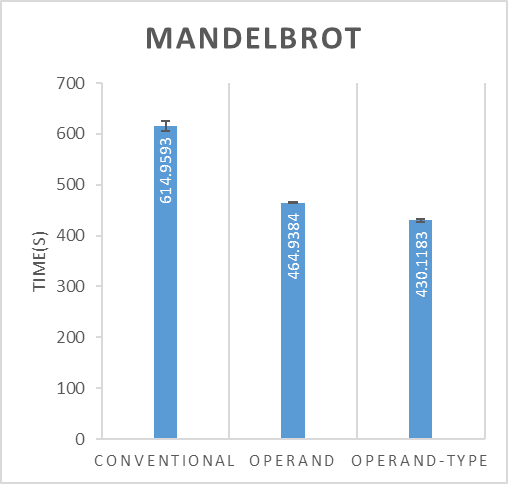
\includegraphics{mandelbrot.png}
  \caption{Mandelbrot Execution Time}
  \label{fig:mandel-time}
\end{figure}

\subsection{Mersenne Twister}
The mersenne twister had a large performance increase relative to
other benchmarks, but experienced the smallest increase for the
Operand-Type Dispatch VM over the Operand VM with a 2.7\% increase.

\subsection{Prime Sieve}
The Prime Sieve benchmark had quite average performance increases
compared to other benchmarks. It also produced an interesting trend of
higher cache-misses for the experimental VMs in the Perf benchmark
results. Prime Sieve made extensive use of a linked list data
structure which does not have the spatial locality of reference
mentioned in section \ref{sec:cache}. Further investigation is
required to determine why this benchmark makes less effective use of
data cache for the experimental VMs.

\subsection{Reverse Complement}
The Reverse Complement benchmark produced high performance inceases
over the Conventional VM with 21.49\% and 23.68\% for the Operand and
Operand-Type VMs respectively. The cache miss rate found by the Perf
utility was high for this benchmark. This is because it is the only
benchmark that reads extensively from standard input. 

\chapter{Conclusion}

The project objective, to implement and benchmark an experimental
JIT-less, dynamic-ISA VM was met. Two experimental VMs, the Operand
Dispatch and and Operand-Type Dispatch VMs were implemented along with
a Conventional VM which served as a control. A set of benchmarks was
handwritten and benchmarked extensively to determine the overall
performance of the experimental VMs.

The Operand and Operand-Type dispatch VMs do indeed present solutions
to the problem of a VM that is appropriate for many-instance
applications that does not make use of a just in time compiler. Both
experimental VMs were faster than the Conventional VM against which
they were benchmarked. The Operand Dispatch VM provided an 8.53\% to
24.4\% increase over a conventional VM implementation and the
Operand-Type dispatch provided an 11.91\% to 30.06\% performance
increase.

For general applications, a JIT compiler implementation would still be
preferred, as the performance benefits offered by the two experimental
VMs do not approach those of a JIT compiler. But for short-lived, many
instance applications, like those of a web server, and in any new
dynamic interpreter implementation where a JIT compiler is not
desired, the techniques used in the Operand and Operand-Type VMs are
worth consideration.

The Operand-Type Dispatch VM did not provide the performance increase
hoped for, with a 2.7\% to 8.53\% increase in performance over the
Operand dispatch VM. A slightly better code generation implementation
(see section \ref{sec:generation-algorithm}) may result in even better
performance for the Operand Dispatch VM. Thus the Operand Dispatch VM
is considered the superior technique because it is less complex to
implement and makes fewer of the trade-offs necessary for the
Operand-Type VM, while still providing most of the performance
benefits gained by the Operand-Type VM.

\bibliographystyle{apacite} 
\bibliography{treatise-bibliography}

\newpage{}
\appendix
\chapter{Project Proposal} 

Present state of the art high-level virtual machines (VMs) utilise
trace-based just-in-time compilers (JITs) to approach native
performance. However, JITs create code in private process memory,
defeating benefits of read-only memory sharing, which is important in
applications that run many concurrent instances. 

This project forms part of a larger research project to investigate
novel innovations to JIT-less VMs which strongly favour run-time
efficiency in many-instance applications. The larger project explores
multiple possible solution strategies. The specific strategy to be
investigated in this sub-project is the creation of a finite state
space for constrained set of dynamic types (int, float, and
other). The VM is always at some location within the state space, and
dynamic changes in the active type-mapping result in VM movement in
the state space. A modified type-state aware VM could dispatch
instructions relative to that state, thereby branching to code
fragments that are specialised to currently active dynamic types. Such
a mechanism could substantially reduce the cost of dynamic typing when
many value-instances are in fact primitives. 

The scope of this project is limited in two ways. Firstly, the
instruction set architecture will be purposely constrained to about
the size of the Lua register VM, which provides 35 basic
operations. Secondly, the implementation concerns type-mapping only,
and does not concern physical register mapping, which is an orthogonal
issue. More specific details are available in the associated Thuthuka
project proposal.

Note that this project should not be confused with the similar project
relating to register-mapping. These projects are sufficiently
different that they cannot share code. However, they may share a
common set of benchmarks

\chapter{Instruction List} 
\label{appendix-b}

\section{Arithmetic Instructions}
\begin{description}
	\item[add] add two integer-valued registers
	
	$add(i, j) := r _{i} \longleftarrow  r _{i} + r_{j} $ \\
	
	\item[addc] add an integer-valued register and a 64-bit integer
	constant
	
	$addc(i, const _{64}) := r _{i} \longleftarrow  r _{i} + const 
	_{64} $ \\
	
	\item[sub] find the difference of two integer-valued registers
	
	$sub(i, j\neq i) := r _{i} \longleftarrow  r _{i} - r _{j} $ \\
	
	\item[csub] subtract an integer-valued register from a 64-bit 
	integer
	constant
	
	$csub(const _{64}, i) := r _{i} \longleftarrow const _{64} - r 
	_{i} $ \\
	
	\item[mul] multiply two integer-valued registers
	
	$mul(i, j) := r _{i} \longleftarrow  r _{i} \cdot r _{j} $ \\
	
	\item[mulc] multiply an integer-valued register by a 64-bit 
	integer
	constant
	
	$mulc(i, const _{64}) := r _{i} \longleftarrow r _{i} \cdot const 
	_{64} $
	
	\item[div] find the quotient and modulus of two integer-valued
	registers
	
	$div(i, j\neq i) :=$ \\
	$ r _{i} \longleftarrow  r _{i} \div r _{j}$ \\
	$ g _{0} \longleftarrow  r _{i} \textbf{ mod } r _{j} $\\
	
	\item[divc] find the quotient and modulus of an integer-valued
	register and a 64-bit integer constant
	
	$div(i, const _{64}) :=$ \\
	$ r _{i} \longleftarrow  r _{i} \div const_{64}$ \\
	$ g _{0} \longleftarrow r _{i} \textbf{ mod } const_{64} $
	
\end{description}

\section{Bit Manipulation Instructions}
\begin{description}
	\item[and] bitwise and two integer-valued registers
	
	$and(i, j\neq i) := r _{i} \longleftarrow  r _{i}  \textbf{ and } 
	r _{j} $ \\
	\item[andc] bitwise and an integer-valued register and 64-bit 
	integer
	constant
	
	$andc(i, const _{64}) :=  r _{i} \longleftarrow  r _{i} \textbf{ 
	and } const _{64} $ \\
	\item[or] bitwise or two integer-valued registers
	
	$or(i, j \neq i) := r _{i} \longleftarrow  r _{i} \textbf{ or } r 
	_{j} $  \\
	\item[orc] bitwise or an integer-valued register and 64-bit 
	integer
	constant
	
	$orc(i, const _{64}) :=  r _{i} \longleftarrow  r _{i} \textbf{ 
	or } const _{64} $ \\
	\item[xor] bitwise xor two integer-valued registers
	
	$xor(i, j \neq i) := r _{i} \longleftarrow  r _{i} \textbf{ \^{} 
	} r _{j} $ \\
	\item[shl] shift an integer-valued register left by another
	integer-valued register
	
	$shl(i, j) := r _{i} \longleftarrow  r _{i} << r _{j} $ \\
	\item[shlc] shift an integer-valued register left by a 16-bit 
	integer
	constant
	
	$shlc(i, const _{16}) :=  r _{i} \longleftarrow  r _{i} << const 
	_{16} $ \\
  \item[cshl] shift a 64-bit integer constant left by an
    integer-valued register
	
	$cshl(const _{64}, i):=  r _{i} \longleftarrow  const _{64} << r 
	_{i}  $ \\
	\item[shr] logical right shift an integer-valued register by 
	another integer-valued register
	
	$shr(i, j) := r _{i} \longleftarrow  r _{i} >> r _{j} $ \\
	\item[shrc] logical right shift an integer-valued register by a 
	16-bit integer constant
	
	$shrc(i, const _{16}) :=  r _{i} \longleftarrow  r _{i} >> const 
	_{16} $ \\
	\item[cshr] logical right shift a 64-bit integer constant by an
	integer-valued register
	
	$cshr(const _{64}, i):=  r _{i} \longleftarrow  const _{64} >> 
	r{i}  $  \\
	\item[sar] arithmetic right shift an integer-valued register by
	another integer-valued register
	
	$sar(i, j) :=  r _{i} \longleftarrow  r _{i} >>> r _{j} $  \\
	\item[sarc] arithmetic right shift an integer-valued register by a
	16-bit integer constant
	
	$sarc(i, const _{16}) :=  r _{i} \longleftarrow  r _{i} >>> const 
	_{16} $ \\
	\item[csar] arithmetic right shift a 64-bit integer constant by an
	integer-valued register
	
	$csar(const _{64}, i):=  r _{i} \longleftarrow  const _{64} >>> r 
	_{i}  $ \\
\end{description}

\section{Data Movement Instructions}
\begin{description}
	\item[mov] move a register over another register
	
	$mov(i, j \neq i) := g_{i} \longleftarrow g_{j} $ \\
	\item[movc] move a 64-bit integer constant over a register
	
	$movc(i, const_{64}):= g_{i} \longleftarrow const_{64} $ \\
	
	\item[movsc]
	
	\item[null] set a register to null
	
	$null(i):= g_{i} \longleftarrow null $ \\
\end{description}

\section{Memory Access}
\begin{description}
	\item[getl] get a local value indexed by a 16-bit integer 
	constant and store it in a register
	
	$getl(i, const_{16}):= g_{i} \longleftarrow mem[fp + const_{16}]$ 
	\\
	\item[setl] set a local variable indexed by a 16-bit integer 
	constant
	to a register's value
	
	$setl(const_{16}, i):= mem[fp + const_{16}] \longleftarrow g_{i}$ 
	\\
	\item[geto] get a value from an object, indexed by an 
	integer-valued
	register and store it in a register
	
	$geto(i, j, k\neq j):= g_{i} \longleftarrow p_{j}[header + 
	r_{k}*sizeof(value)]$ \\
	\item[seto] set a value, indexed by an integer-valued register, 
	in an
	object to that of a register
	
	$seto(i, j \neq i, k):= p_{i}[header + r_{j}*scale] 
	\longleftarrow g_{k}$ \\
	\item[getb] get a value from a buffer, indexed by an 
	integer-valued
	register and store it in a register
	
	$getb(i, j, k\neq j):= g_{i} \longleftarrow p_{j}[header + 
	r_{k}*sizeof(int8\_t)]$ \\
	\item[setb] set a value, indexed by an integer-valued register, 
	in a
	buffer to that of a register
	
	$setb(i, j \neq i, k):= p_{i}[header + r_{j}*scale] 
	\longleftarrow r_{k}$ \\
\end{description}

\section{Control Flow Instructions}
\begin{description}
	\item[jmp] adds a 16-bit integer constant offset to \verb|IP|
	
	$jmp(const_{16}) := ip \longleftarrow ip + const_{16}$ \\
	\item[jmpf] adds a 64-bit integer constant offset to \verb|IP|
	
	$jmpf(const_{64}) := ip \longleftarrow ip + const_{64}$ \\
	\item[switch]
	
	$switch := todo: me$ \\
	\item[jcmp] adds one of three 16-bit integer constant offsets to
	\verb|IP| depending on which case holds for two different
	integer-valued registers
	
	$jcmp(i, j\neq i,less_{16},equal_{16},greater_{16}) :=$ \\
	$ ip \longleftarrow  \\
	case :r_{i} < r_{j}: ip + less_{16}   \\
	case :r_{i} = r_{j}: ip + equal_{16} \\
	case :r_{i} > r_{j}: ip + greater_{16}$ \\
	\item[jcmpc] adds one of three 16-bit integer constant offsets to
	\verb|IP| depending on which case holds for an integer-valued
	register and 64-bit integer constant
	
	$jcmpc (i, const_{64},less_{16},equal_{16},greater_{16}) :=$ \\
	$ ip \longleftarrow  \\
	case: r_{i} < const_{64}: ip + less_{16}   \\
	case: r_{i} = const_{64}: ip + equal_{16} \\
	case: r_{i} > const_{64}: ip + greater_{16}$
	\item[jnullp] adds one of two 16-bit integer constant offsets to
	\verb|IP| depending on if a pointer-valued register is null or not
	
	$jnullp(i,not-null-disp16,null-disp16) :=$ \\
	$ip \longleftarrow \\
	case: p_{i} \neq null: ip + not-null-disp_{16} \\
	case: p_{i} = null: ip + null-disp_{16}$ \\
\end{description}

\section{Function Call and Return}
\begin{description}
	\item[call] sets up a new stack frame, saves the old state of the 
	VM
	before the call, copies arguments and moves execution to the
	function's instructions
	
	$call(disp_{16}, first_{16}, count_{16}) :=$ \\
	$newip \longleftarrow ip + disp_{16};\\
	locals\_size \longleftarrow *(int64\_t *)newip\\
	size \longleftarrow sizeof(stackframe) + sizeof(value) * 
	locals\_size;\\
	stackframe *base \longleftarrow (stackframe*)malloc(size);\\
	base \longleftarrow stackframe\_new(fp, ip, ts, g, first_{16}, 
	count_{16}); \\
	fp \longleftarrow base->l \\
	ip \longleftarrow newip + 4 \\
	$\\
	First the variable $newip$ is created which is the location of the
	function definition of the function being called. At that position
	is a 64-bit integer which contains the count of the number of 
	local
	variables used by the function. This count is stored in the
	variable: $locals\_size$. A new stack frame of the correct size is
	allocated. The value returned by malloc for this allocation is
	called $base$ because it is a pointer that points to the base of 
	the
	new stack frame.
	
	The code for initialising the stack frame has been omitted in the
	interest of brevity but shall be described here. For reference,
	figure~\ref{fig:stframe} gives a visual representation of the 
	fields
	of the stack frame. The current frame's \verb|FP|, \verb|IP|,
	\verb|TS| and registers $g_1$ through $g_4$ are stored in the new
	stack frame using simple assignment.
	
	Next, the function's arguments are copied over to the start of the
	new stack frame's local variables using memcpy. The first argument
	is the local variable in the current stack frame indexed by
	$first_{16}$ and the number of arguments is $count_{16}$. The rest
	of the local variables are those needed by the function to perform
	its tasks.
	
	The \verb|FP| can now be updated to point to the local variables 
	of
	the current stack frame and the \verb|IP| is set to the newip 
	value
	with 4 instruction words skipped to point to the first instruction
	after the 64-bit integer.
	
	\item[ret] restores the previous stack frame and frees the current
	stack frame
	$ret() := $  \\
	$ stackframe *cur \longleftarrow (stackframe*)((size\_t)fp - 
	sizeof(stackframe)) \\
	fp \longleftarrow cur.fp \\
	ip \longleftarrow cur.ip \\
	RestoreTS(cur.ts, ts);\\
	RestoreRegisters(cur.g) \\
	free(cur); \\$
	
	First the address of the current stack frame is aquired and stored
	in $cur$.
	Next the saved values for FP, IP, TS and g1 through g4 are 
	restored.
	Finally the current stack frame is freed.
\end{description}

\section{Pragmatic Higher-Level Instructions}

\begin{description}
	\item[newo] allocates a new object of size given by an 
	integer-valued
	register and assigns it to some register
	
	$ newo(i, j \neq i) := $ \\
	$  object *base \longleftarrow (object*)malloc(sizeof(object) + 
	sizeof(value)* r_j) \\
	base.size \longleftarrow r_i\\
	g_i \longleftarrow base \\ $
	
	\item[newb]{} allocates a new object of size given by an
	integer-valued register and assigns it to some register
	
	$ newb(i, j \neq i) := $ \\
	$  object *base \longleftarrow (buffer*)malloc(sizeof(object) + 
	sizeof(int8\_t)* r_j) \\
	base.size \longleftarrow r_i\\
	g_i \longleftarrow base \\ $
	
	\item[err] prints an error string at a 16-bit integer value
	displacement from IP then halts VM
	
	% movsc goes here???
	
	\item[in] attempts to fill a buffer from standard input
	
	\item[out] writes out a stream of data from a buffer to stdout
	
	\item[print] writes a line of data to stdout
	
\end{description}
\chapter{Macros}

Several macros are used to make the source code more readable and code
generation less verbose. The reader may wish to know the precise
definitions of these macros. The full list of macros is presented here
for conveniece.

\section{Stack Frame Macros}
\label{sec:stackframemacros}
These macros are used to save and restore registers between stack
frames and to restore the \verb|TS| register.

\begin{lstlisting}
#define SaveRegisters(saveg, oldg) {saveg[0] = oldg[1]; saveg[1] = oldg[2]; saveg[2] = oldg[3]; saveg[3] = oldg[4];}
#define RestoreRegisters(saveg, oldg) {oldg[1] = saveg[0]; oldg[2] = saveg[1]; oldg[3] = saveg[2]; oldg[4] = saveg[3];}
#define RestoreTS(curTS, TS) (TS = (curTS & 0xF000) | (TS & 0x10800))
\end{lstlisting}

\section{Conventional VM Macros}
\label{sec:convmacros}

These macros are used to get arguments and opcodes from instruction
words in the Conventional VM. They are also used to check the types of
registers which the Operand Dispatch VM also makes use of.

\begin{lstlisting}
#define GetArg0(inst) ((inst) & 0x7) 
#define GetArg1(inst) (((inst) & 0x38) >> 0x3)
#define GetArg2(inst) (((inst) & 0x1FF) >> 0x6) 

#define IsInt(x) ((x).tag == 0)
#define IsPointer(x) ((x).tag >= 1)
#define GetOpcode(inst) ((inst) >> 0x9)
\end{lstlisting}

\section{Data Type Macros}
\label{sec:datamacros}
These macros are used to maintain and access the size and flags field
of objects and buffers.

\begin{lstlisting}
#define MakeSizeAndFlags(size,flags)(((size)<<2)|(flags))
#define GetFlags(v)((v) & 3)
#define GetSize(v)((v) >> 2)
\end{lstlisting}

\chapter{Results Data}

Average execution time is in seconds. Values in round brackets are the
standard deviations of the rates as percentage points. Values in
square brackets are paired, two-tailed T test results for the two sets
the speed increase applies to.

\section{Benchmark Result Tables}
\begin{table}[!htb]
  \begin{center}
    \begin{tabular}{lrrr}
      Ackermann & Conventional & Operand & Operand-Type\\
      \hline
      Average execution time & 125.7464 & 115.5056 & 110.7639\\
      Increase over Conventional &  & 8.14\% [3.85E-23] & 11.91\% [7.23E-17]\\
      Increase over Operand &  &  & 4.11\% [2.08E-5]\\
      Perf cache-miss & 14.76\% (1.06\%) & 14.51\% (0.66\%) & 14.87\% (0.94\%)\\
      Perf branch-miss & 0\% (0\%) & 0\% (0\%) & 0\% (0\%)\\
      Cachegrind I1 miss & 0\% & 0\% & 0\%\\
      Cachegrind indirect miss & 58.3\% & 8.3\% & 8.3\%\\
    \end{tabular}
  \end{center}
  \caption{Ackermann}
\end{table}

\begin{table}[!htb]
  \begin{center}
    \begin{tabular}{lrrr}
      Fannkuch & Conventional & Operand & Operand-Type\\
      \hline
      Average execution time & 47.1528 & 39.0194 & 35.6915\\
      Increase over Conventional &  & 17.25\% [1.54E-39] & 24.31\% [1.02E-38]\\
      Increase over Operand &  &  & 8.53\% [6.11E-21]\\
      Perf cache-miss & 5.12\% (2.17\%) & 5.46\% (1.29\%) & 10.40\% (7.71\%)\\
      Perf branch-miss & 0.61\% (0.01\%) & 0.74\% (0.03\%) & 0.97\% (0.02\%)\\
      Cachegrind I1 miss & 0\% & 0\% & 0\%\\
      Cachegrind indirect miss & 73.2\% & 22.7\% & 23.3\%\\
    \end{tabular}
  \end{center}
  \caption{Fannkuch}
\end{table}

\begin{table}[!htb]
  \begin{center}
    \begin{tabular}{lrrr}
      Fasta & Conventional & Operand & Operand-Type\\
      \hline
      Average execution time & 54.9107 & 46.622 & 44.6889\\
      Increase over Conventional &  & 15.09\% [2.08E-8] & 18.62\% [4.55E-00]\\
      Increase over Operand &  &  & 4.15\% [0.0015]\\
      Perf cache-miss & 3.44\% (2.00\%) & 4.05\% (1.79\%) & 5.29\% (3.30\%)\\
      Perf branch-miss & 0.25\% (0.06\%) & 0.26\% (0.00\%) & 0.39\% (0.04\%)\\
      Cachegrind I1 miss & 0\% & 0\% & 0\%\\
      Cachegrind indirect miss & 74.3\% & 22.5\% & 24.1\%\\
    \end{tabular}
  \end{center}
  \caption{Fasta}
\end{table}

\begin{table}[!htb]
  \begin{center}
    \begin{tabular}{lrrr}
      Mandelbrot & Conventional & Operand & Operand-Type\\
      \hline
      Average execution time & 614.9593 & 464.9384 & 430.1183\\
      Increase over Conventional &  & 24.40\% [3.58E-12] & 30.06\% [8.91E-13]\\
      Increase over Operand &  &  & 7.49\% [6.77E-11]\\
      Perf cache-miss & 6.99\% (2.41\%) & 6.53\% (2.90\%) & 8.20\% (2.07\%)\\
      Perf branch-miss & 0.04\% (0.00\%) & 0.05\% (0.00\%) & 0.11\% (0.00\%)\\
      Cachegrind I1 miss & 0\% & 0\% & 0\%\\
      Cachegrind indirect miss & 85.7\% & 29.6\% & 36.6\%\\
    \end{tabular}
  \end{center}
  \caption{Mandelbrot}
\end{table}

\begin{table}[!htb]
  \begin{center}
    \begin{tabular}{lrrr}
      Mersenne Twister & Conventional & Operand & Operand-Type\\
      \hline
      Average execution time & 30.4329 & 24.3093 & 23.6524\\
      Increase over Conventional &  & 20.12\% [2.31E-8] & 22.28\% [1.30E-7]\\
      Increase over Operand &  &  & 2.70\% [0.0148]\\
      Perf cache-miss & 4.41\% (2.78\%) & 4.63\% (1.93\%) & 4.01\% (1.18\%)\\
      Perf branch-miss & 0.44\% (0.15\%) & 0.44\% (0.08\%) & 0.63\% (0.06\%)\\
      Cachegrind I1 miss & 0\% & 0\% & 0\%\\
      Cachegrind indirect miss & 64.9\% & 24\% & 24.6\%\\
    \end{tabular}
  \end{center}
  \caption{Mersenne Twister}
\end{table}

\begin{table}[!htb]
  \begin{center}
    \begin{tabular}{lrrr}
      Prime Sieve & Conventional & Operand & Operand-Type\\
      \hline
      Average execution time & 193.9987 & 160.2169 & 152.4721\\
      Increase over Conventional &  & 17.41\% [1.79E-10] & 21.41\% [4.76E-12]\\
      Increase over Operand &  &  & 4.83\% [0.0005]\\
      Perf cache-miss & 15.87\% (0.34\%) & 16.48\% (0.32\%) & 23.11\% (2.17\%)\\
      Perf branch-miss & 0.00\% (0.00\%) & 0.00\% (0.00\%) & 0.00\% (0.00\%)\\
      Cachegrind I1 miss & 0\% & 0\% & 0\%\\
      Cachegrind indirect miss & 81.8\% & 27.2\% & 27.2\%\\
    \end{tabular}
  \end{center}
  \caption{Prime Sieve}
\end{table}

\begin{table}[!htb]
  \begin{center}
    \begin{tabular}{lrrr}
      Reverse Complement & Conventional & Operand & Operand-Type\\
      \hline
      Average execution time & 2.6406 & 2.0731 & 2.01531\\
      Increase over Conventional &  & 21.49\% [3.25E-50] & 23.68\% [1.71E-52]\\
      Increase over Operand &  &  & 2.79\% [1.61E-10]\\
      Perf cache-miss & 39.63\% (4.72\%) & 42.99\% (4.46\%) & 39.83\% (5.20\%)\\
      Perf branch-miss & 0.10\% (0.01\%) & 0.11\% (0.00\%) & 1.70\% (1.09\%)\\
      Cachegrind I1 miss & 0\% & 0\% & 0\%\\
      Cachegrind indirect miss & 44.6\% & 1.6\% & 1.6\%\\
    \end{tabular}
  \end{center}
  \caption{Reverse Complement}
\end{table}

\section{Execution Times}

\begin{figure}[!htb]
  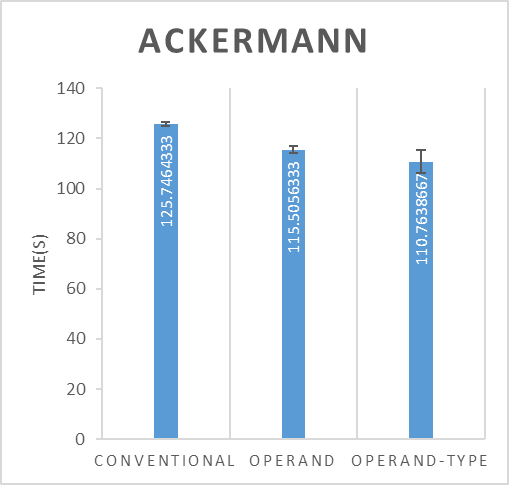
\includegraphics{ackermann.png}
  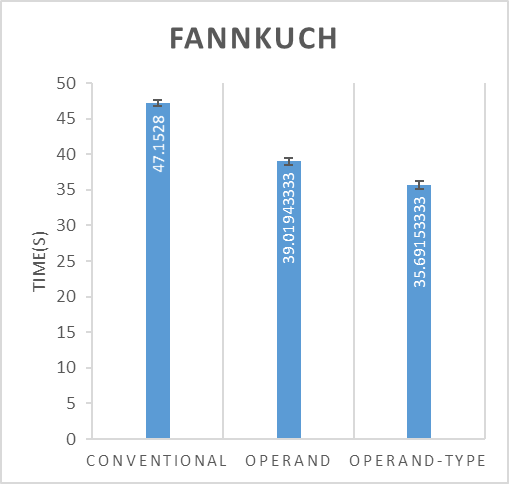
\includegraphics{fannkuch.png} 
  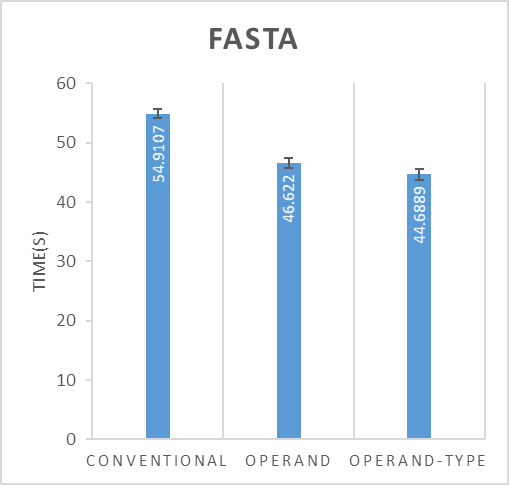
\includegraphics{fasta.png}
  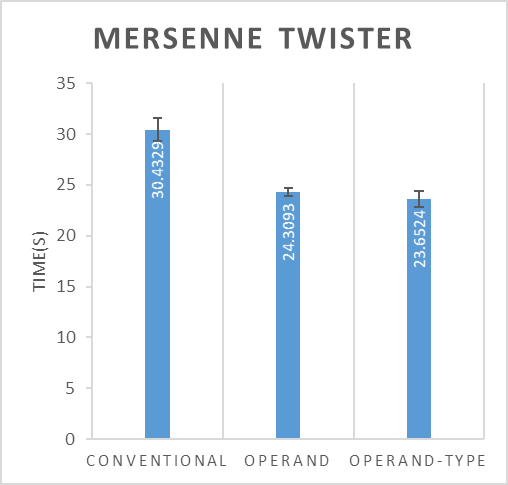
\includegraphics{mersenne.png}
  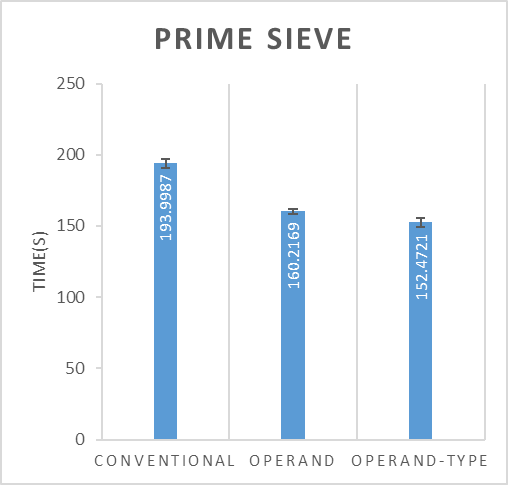
\includegraphics{primesieve.png}
  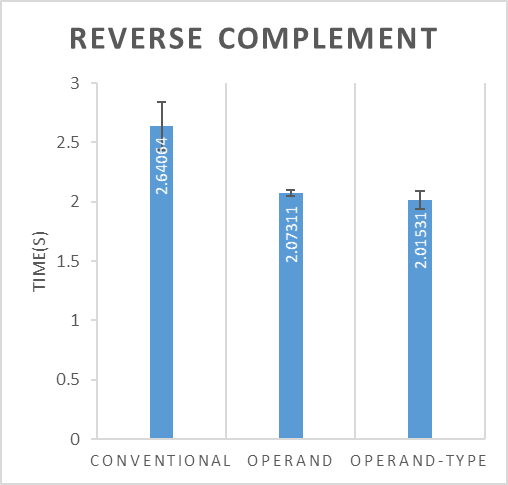
\includegraphics{reversecomplement.png}
  \caption{Execution Time of Remaining Benchmarks}
  \label{execution-time}
\end{figure}




\end{document}


